\documentclass[11pt,a4paper]{article}

\usepackage[utf8]{inputenc}
\usepackage[T1]{fontenc}
\usepackage{lmodern}
\usepackage{microtype}
\usepackage[margin=1in]{geometry}
\usepackage{setspace}
\onehalfspacing

\usepackage{amsmath,amssymb,mathtools,amsthm}
\usepackage{graphicx}
\usepackage{flafter}
\usepackage{placeins}
\usepackage{xcolor}
\usepackage{booktabs,array}
\usepackage[ruled,vlined,linesnumbered]{algorithm2e}
\usepackage[round,authoryear]{natbib}
\usepackage{url}
\usepackage[colorlinks=true,linkcolor=blue!60!black,citecolor=blue!60!black,urlcolor=blue!60!black,pdftitle={The Epistemic Fluency Trap in AI-Augmented Security Operations},pdfauthor={Author Blinded for Review}]{hyperref}
\usepackage[capitalize,nameinlink,noabbrev]{cleveref}

\renewcommand{\topfraction}{0.95}
\renewcommand{\bottomfraction}{0.92}
\renewcommand{\textfraction}{0.05}
\renewcommand{\floatpagefraction}{0.88}
\setcounter{topnumber}{3}
\setcounter{bottomnumber}{2}
\setcounter{totalnumber}{4}
\setlength{\textfloatsep}{10pt plus 2pt minus 2pt}
\setlength{\floatsep}{8pt plus 2pt minus 2pt}
\setlength{\intextsep}{10pt plus 2pt minus 2pt}

\newcolumntype{L}[1]{>{\raggedright\arraybackslash}p{#1}}
\let\oldtexttt\texttt
\renewcommand{\texttt}[1]{\textnormal{\oldtexttt{#1}}}

\newtheorem{proposition}{Proposition}
\newtheorem{theorem}{Theorem}
\newtheorem{corollary}{Corollary}
\newtheorem{definition}{Definition}
\crefname{proposition}{Proposition}{Propositions}
\Crefname{proposition}{Proposition}{Propositions}
\crefname{theorem}{Theorem}{Theorems}
\Crefname{theorem}{Theorem}{Theorems}
\crefname{corollary}{Corollary}{Corollaries}
\Crefname{corollary}{Corollary}{Corollaries}
\crefname{algocf}{Algorithm}{Algorithms}
\Crefname{algocf}{Algorithm}{Algorithms}
\crefname{algorithm}{Algorithm}{Algorithms}
\Crefname{algorithm}{Algorithm}{Algorithms}

\title{\textbf{The Epistemic Fluency Trap in AI-Augmented Security Operations: Generative Rationale Fluency, Telemetry Partitioning, and Defeasible Contestation}}

\author{
  Author Blinded for Review\\
  \small Submitted to \textit{Journal of Management Information Systems}
}
\date{October 2026}

\begin{document}

\maketitle

\begin{abstract}
Enterprise Security Operations Centers (SOCs) increasingly embed large language model (LLM) copilots into SIEM and XDR workflows to synthesize heterogeneous telemetry into natural-language triage rationales. Although prevailing Information Systems (IS) scholarship assumes that explanation coherence monotonically improves human sensemaking and trust calibration, this assumption breaks down in high-velocity, adversarially contested security environments. Drawing on metacognitive processing fluency theory, cognitive fit theory, and Toulmin's model of defeasible argumentation, we formulate a normative analytical governance framework, the \textbf{Dual-Cue Epistemic Defeasibility Model (DCEDM)}, and design a computational design science countermeasure pairing the \textbf{Prompt-Isolated Telemetry Discrepancy Scorer (PITSA)} with a Two-Stage \textbf{Defeasible Epistemic Cueing System (DECS)}. Grounded in three generalizable socio-technical design principles and partitioned strictly over kernel and network structural attributes while excluding untrusted command-line and alert text, PITSA computes an additive empirical log-likelihood ratio that triggers a selective Toulmin rebuttal cue only when primary structural telemetry contradicts a benign AI disposition. We evaluate DCEDM and PITSA/DECS through a four-part empirical and trace-driven decision-theoretic design across $2,238,434$ real telemetry records ($671,531$ held-out test records) and $1,741$ actively exploited vulnerabilities: (1) host-level attack-replay evaluation on the Open Threat Research Forge (OTRF) Security-Datasets corpus ($N = 43,723$ Windows Sysmon/Security events across 63 archives); (2) enterprise SIEM alert evaluation on the SALAD-SOC benchmark ($N = 416,781$ labeled alerts); (3) large-scale lateral-movement evaluation on the LMD-2023 Sysmon corpus ($N = 1,777,930$ rows) and CISA KEV catalog ($N = 1,741$ CVEs); and (4) trace-driven analytical Bayesian decision-theoretic sensitivity and endogenous habituation analysis across four governance policies. Under both graded appended ($m \in \{1, 2, 4, 8\}$ benign clauses appended to preserved malicious text) and full-override Indirect Telemetry Prompt Injection (ITPI), five unpartitioned text-inclusive baselines spanning classical lexical, dense semantic neural MLP, and contextual subword language model architectures suffer severe recall collapse on OTRF ($85.81\% \to 30.32\%$ under appended ITPI and $25.16\%$ under full ITPI for Logistic Regression; $65.81\% \to 8.39\% \to 0.00\%$ for Dense Neural MLP; $74.19\% \to 0.00\%$ for Naive Bayes) and SALAD-SOC ($77.46\%\text{ to }84.93\%$ clean recall dropping to $2.92\%\text{ to }36.05\%$ under ITPI; McNemar's $\chi^2 \ge 8,361.46, p < 0.0001$), whereas Partitioned PITSA remains strictly invariant ($0.00$ percentage point recall drop), achieving $\text{AUROC} = 0.9807$ ($95\%\text{ CI}: [0.9685, 0.9901]$) on OTRF, $\text{AUROC} = 0.9380$ ($95\%\text{ CI}: [0.9324, 0.9401]$, with $98.14\%$ to $99.66\%$ recall across Execution, Persistence, and Reconnaissance tactics) on SALAD-SOC, and $\text{AUROC} = 0.9963$ ($95\%\text{ CI}: [0.9961, 0.9969]$, $99.93\%$ hostile recall, $99.99\%$ RedTeam recall) on LMD-2023. Trace-driven decision-theoretic evaluation identifies the exact cost-ratio dominance boundary ($\kappa^* = 39.64$ on low-base-rate OTRF vs.\ $\kappa^* = 1.68$ on SALAD-SOC at $\lambda_F = 0.40$), establishes an interior optimal gating threshold under unified endogenous habituation, and shows that selective DECS gating cuts warning banner volume by $79.87\%$ to $95.92\%$ while reducing expected operational loss by $30.16\%$ to $60.77\%$ in enterprise SIEM triage.
\end{abstract}

\medskip
\noindent\textbf{Keywords:} Epistemic fluency trap; human-AI delegation; security operations center (SOC); computational design science; defeasible argumentation; decision-theoretic governance; indirect telemetry prompt injection (ITPI).

\section{Introduction}
\label{sec:intro}

\subsection{Phenomenon and Practical Stakes in AI-Augmented Security Operations}
\label{subsec:phenomenon}

Contemporary enterprise Security Operations Centers (SOCs) operate under an acute structural tension between exponentially expanding telemetry volume and finite analytical capacity \citep{tariq2025alert, tilbury2024automation, bartal2026alert}. Modern Security Information and Event Management (SIEM) and Extended Detection and Response (XDR) platforms ingest millions of host, identity, and network events daily, subjecting Tier-1 and Tier-2 triage workflows to severe alert fatigue, cognitive overload, and service-level agreement (SLA) time pressure \citep{cram2021technostress, hsu2024proactive, darcy2014stress, liu2020centralized}. To strengthen enterprise infrastructure resilience \citep{li2021roles, ebrahimi2020semi, ampel2024improving}, organizations have rapidly deployed generative artificial intelligence (AI) copilots, including Microsoft Security Copilot, CrowdStrike Charlotte AI, and Google Chronicle Gemini, directly into the operational triage loop \citep{srinivas2025ai, ansari2026partner}. Unlike legacy rule-based prioritizers or black-box anomaly classifiers that output opaque numerical risk scores \citep{li2022assessing, tutun2024explainable}, generative AI copilots translate fragmented kernel and network telemetry into fluent, grammatically cohesive natural-language narratives that explain why an alert was triggered and recommend whether to escalate or dismiss the incident \citep{naseer2023enabling, bag2025enhancing, taudien2026effect}.

Although embedding natural-language explanations alongside AI triage recommendations is intended to resolve the opacity dilemma in human-AI collaboration \citep{lebovitz2022engage, fugener2022cognitive, revilla2023human} and keep the human expert ``in the loop'' as the final institutional gatekeeper \citep{baird2021next, raisch2021artificial, ansari2026partner}, a critical socio-technical vulnerability persists in live SOC workflows. Field evidence and emerging behavioral security critiques indicate that the very linguistic coherence that reduces reading effort can simultaneously disarm the forensic interrogation practices on which human-in-the-loop security governance depends \citep{tilbury2024automation, bucinca2021trust, bag2025enhancing}. When a generative copilot presents a polished, internally consistent narrative attributing a suspicious process execution to routine administrative maintenance, time-pressed decision-makers face strong cognitive incentives to treat the narrative as a verified synthesis of the underlying logs and close the incident ticket without inspecting the primary forensic telemetry \citep{vasconcelos2023explanations, tariq2025alert, bartal2026alert}. As a consequence, erroneous or adversarially manipulated AI dismissals can pass unchallenged through review, creating an urgent need to formalize how linguistic presentation fluency and architectural telemetry partitioning govern primary evidentiary verification.

\subsection{The Theoretical Paradox: Generative Explainability as an Epistemic Sedative}
\label{subsec:paradox}

Following the problematization mandate in Information Systems scholarship \citep{chatterjee2020need, diaz2023indigenous}, we challenge a foundational assumption shared across the IS, decision support, and Human-Computer Interaction (HCI) literatures on explainable AI (XAI): namely, that increasing the interpretability and linguistic coherence of an AI explanation monotonically supports sensemaking and appropriate trust calibration \citep{burton2020systematic, jussupow2021augmenting, tutun2024explainable, bag2025enhancing, taudien2026effect}. Recent decision-support research demonstrates that LLM-generated narrative explanations measurably improve subjective comprehension for non-expert and operational users \citep{bag2025enhancing}, while meta-analytic and empirical studies of human-AI partnerships show that explanation interfaces shape whether humans treat AI as a subordinate tool or an authoritative partner \citep{ansari2026partner, revilla2023human, baird2021next, fugener2021will}. Under this prevailing transparency paradigm, verification failures are attributed primarily to algorithmic opacity (``black boxes'') or uncalibrated user metaknowledge \citep{lebovitz2022engage, fugener2022cognitive, tutun2024explainable}.

We argue that this transparency assumption breaks down in high-velocity, adversarially contested data environments because it conflates \textit{subjective processing fluency} with \textit{evidentiary warrant}. Drawing on metacognitive processing fluency theory \citep{alter2009uniting}, evaluators routinely substitute the cognitive ease of processing an explanation for the truth value and evidentiary completeness of its underlying claim. When an LLM summarizes noisy multi-event telemetry into continuous prose, it performs what we term \textit{epistemic smoothing}: it resolves forensic ambiguity in favor of a single dominant storyline, omits low-salience structural anomalies that conflict with the narrative arc, and presents its conclusion with uniform rhetorical confidence. In contrast, structured telegraphic summaries that preserve raw field-value tokens impose deliberate perceptual disfluency, signaling that the summary is an incomplete index requiring primary log verification. Consequently, rather than functioning as a scaffold for critical evaluation, high generative fluency acts as an \textit{epistemic sedative} that prematurely satisfies the threshold for causal coherence and suppresses drill-down into primary telemetry.

\subsection{Adversarial Amplifier: Indirect Telemetry Prompt Injection (ITPI)}
\label{subsec:itpi}

This cognitive and architectural vulnerability becomes an acute enterprise security risk when exploited by an emerging class of adversarial manipulation that we formalize as \textbf{Indirect Telemetry Prompt Injection (ITPI)} \citep{srinivas2025ai, ampel2024improving}. In an enterprise SOC telemetry pipeline, an LLM copilot or unpartitioned triage classifier constructs its assessment by ingesting both kernel-enforced structural telemetry attributes ($\mathcal{A}_{\text{struct}}$, such as Sysmon Event IDs, parent-child process lineage, binary signature status, integrity levels, network flow volumes, and destination ports) and untrusted text fields controlled by the monitored endpoint or external network actor ($\mathcal{A}_{\text{text}}$, such as command-line arguments, PowerShell script comments, HTTP user-agent strings, and SIEM alert description strings). Because standard summarization and classification pipelines concatenate these heterogeneous fields into a unified feature or prompt context, an adversary who executes a malicious payload on a compromised host can simultaneously append or inject a plausible benign administrative rationale or routine traffic banner inside the untrusted text string.

When an unpartitioned classifier or LLM copilot ingests this poisoned telemetry stream, the embedded benign text tokens shift the model's posterior probability and sequence representation toward a fluent, reassuring benign disposition (for example, characterizing an unsigned \texttt{rundll32.exe} process opening a reading handle to \texttt{lsass.exe} memory as a sanctioned enterprise single-sign-on diagnostic utility). At the kernel and network header layers, the raw structural telemetry recorded by the operating system and flow sensors remains intact, exhibiting high-severity indicators of credential dumping (Sysmon Event ID 10), process injection (Sysmon Event ID 8), or lateral movement (Sysmon Event ID 3). However, if the verification monitor itself ingests $\mathcal{A}_{\text{text}}$, or if the fluent narrative suppresses raw log inspection, the contradiction between the benign text narrative and the hostile structural telemetry goes undetected. ITPI thus exploits the socio-technical seam between an unpartitioned model's susceptibility to untrusted text context and the decision-maker's susceptibility to narrative fluency.

\subsection{Research Questions and Core Contributions}
\label{subsec:rqs_contributions}

Given the unresolved gap regarding how untrusted text channels and generative linguistic fluency degrade adversarial triage resilience, and how selective conflict cueing can restore verification without inducing neuro-cognitive warning habituation \citep{anderson2016warning, vance2018fog, jensen2022improving}, this study addresses three linked research questions:
\begin{itemize}
  \item \textbf{RQ1 (Architectural Vulnerability vs.\ Partitioned Invariance):} To what extent does ingesting untrusted telemetry text ($\mathcal{A}_{\text{text}}$) alongside structural attributes ($\mathcal{A}_{\text{struct}}$) expose unpartitioned triage classifiers (across classical lexical, dense semantic neural, and contextual subword language model architectures) to recall collapse under both graded appended and full-override Indirect Telemetry Prompt Injection (ITPI), and can a strictly partitioned white-box log-likelihood ratio scorer (PITSA) maintain high discriminative accuracy across heterogeneous host and network telemetry corpora?
  \item \textbf{RQ2 (Normative Decision-Theoretic Mechanism and Dominance Boundaries of DCEDM):} Within a normative Bayesian decision-theoretic governance model of SLA-constrained alert triage (DCEDM), how does narrative fluency inflation ($\tilde{F} > F_0$) distort posterior compromise beliefs and inflate expected Compromise Miss Rates (CMR), and what are the exact cost-ratio crossover boundaries ($\kappa^*$) and endogenous habituation conditions under which selective contestation dominates or underperforms unassisted triage?
  \item \textbf{RQ3 (Selective Socio-Technical Governance via DECS):} Driven by real held-out telemetry streams, how does a Two-Stage Defeasible Epistemic Cueing System (DECS) gated by PITSA compare against unassisted fluent triage and static persistent warning banners in bounding warning habituation, optimizing interior gating thresholds ($\tau^*_{\text{LLR}}$), and minimizing expected operational loss across asymmetric cost regimes?
\end{itemize}

Our central thesis is that unpartitioned text ingestion and high explanation fluency in security operations create a dual socio-technical vulnerability to Indirect Telemetry Prompt Injection, but that strictly partitioning structural telemetry from untrusted text to trigger selective, white-box Toulmin rebuttal cues preserves detection invariance and minimizes expected operational loss within clearly defined cost-ratio boundaries. Specifically, we contribute: (1) the \textbf{Dual-Cue Epistemic Defeasibility Model (DCEDM)}, a normative Bayesian decision-theoretic governance model that advances IS human-AI delegation and explainability theory \citep{baird2021next, fugener2022cognitive, revilla2023human, ansari2026partner, bag2025enhancing} by formally deriving how fluency-weighted belief distortion compresses optimal verification effort under SLA constraints (\cref{thm:dcedm_dominance}) and characterizing the exact cost-ratio dominance boundary $\kappa^*$ and interior optimal threshold $\tau^*_{\text{LLR}}$ under unified endogenous warning habituation (\cref{cor:dominance_boundary}); (2) the \textbf{Prompt-Isolated Telemetry Discrepancy Scorer (PITSA)} and \textbf{Two-Stage DECS} artifact, grounded in three generalizable socio-technical design principles (\textbf{DP1 to DP3}) for computational security design science \citep{ebrahimi2020semi, li2022assessing, ampel2024improving, tutun2024explainable}, which enforces an architectural air-gap between $\mathcal{A}_{\text{struct}}$ and $\mathcal{A}_{\text{text}}$ (\cref{prop:partition_invariance}) while providing exact per-pillar forensic attribution in microseconds per event on a single CPU; and (3) a four-part multi-corpus empirical and trace-driven decision-theoretic evaluation across $2,238,434$ real telemetry records (\texttt{OTRF Security-Datasets}, \texttt{SALAD-SOC}, and \texttt{LMD-2023}) and $1,741$ \texttt{CISA KEV} vulnerabilities comparing Partitioned PITSA against five unpartitioned lexical, dense neural, and subword language model baselines under graded appended and full-override ITPI, alongside adaptive Living-off-the-Land (LOLBin) structural masking.

\section{Theoretical Background and Literature Review}
\label{sec:literature}

\subsection{Human-AI Collaboration, Delegation, and Opacity in Information Systems}
\label{subsec:lit_delegation}

To situate our investigation within the Information Systems and decision-support disciplines, we synthesize three intersecting research streams: (A) human-AI delegation and evidentiary interrogation in IS, (B) metacognitive processing fluency and defeasible argumentation in XAI, and (C) computational cybersecurity design science, behavioral warning habituation, and adversarial telemetry manipulation in SOCs. Within Stream A, IS scholarship has shifted from studying passive decision support tools to theorizing active delegation and role dynamics between human professionals and agentic IS artifacts \citep{baird2021next, raisch2021artificial, revilla2023human, ansari2026partner}. In their foundational framework, \citet{baird2021next} conceptualize delegation as a dynamic transfer of rights and responsibilities between human actors and autonomous or semi-autonomous IS artifacts, emphasizing that effective governance requires aligning decision rights with verification capabilities. Recent research in \textit{Journal of Management Information Systems} underscores the complexity of this alignment: \citet{revilla2023human} demonstrate in operational decision-making that human intervention over algorithmic recommendations is bounded by situational ambiguity and cognitive load, while \citet{ansari2026partner} synthesize through a comprehensive meta-analysis how structural task design determines whether humans engage AI as a verifiable tool or defer to it as an unchallenged partner. Complementary experimental studies confirm that combining human domain experts with high-performing AI models does not automatically yield complementary team performance \citep{fugener2021will, fugener2022cognitive, jussupow2021augmenting}, because humans frequently lack calibrated metaknowledge regarding when their own judgment supersedes the algorithm's inference \citep{fugener2022cognitive} and lose knowledge diversity when exposed to uniform AI advice \citep{fugener2021will}.

In high-stakes diagnostic settings, \citet{lebovitz2022engage} reveal through an ethnographic study of medical radiologists that professionals confronting opaque AI outputs must enact active \textit{interrogation practices}, juxtaposing AI predictions against independent primary evidence rather than passively accepting or rejecting model outputs. In clinical decision-making, \citet{jussupow2021augmenting} trace how diagnostic errors emerge when physicians fail to cross-check algorithmic cues against raw clinical data during hypothesis generation. Extending this stream, \citet{tutun2024explainable} establish in \textit{JMIS} that domain-grounded, white-box explainable decision support is essential for diagnostic sensemaking, and \citet{taudien2026effect} show that providing complementary system information alongside AI predictions can improve delegation effectiveness when supplementary cues accurately reflect underlying uncertainty. Yet existing IS delegation models predominantly examine benign task environments where the AI system's explanation is an honest reflection of its internal reasoning \citep{burton2020systematic, tutun2024explainable, taudien2026effect}. They do not account for socio-technical settings in which the explanation channel itself is subject to generative narrative smoothing or adversarial manipulation.

\subsection{Processing Fluency, Cognitive Forcing, and Defeasible Argumentation}
\label{subsec:lit_fluency}

Turning to the second stream, we integrate insights from metacognitive processing fluency theory \citep{alter2009uniting}, narrative XAI decision support \citep{bag2025enhancing}, and HCI research on overreliance in explainable AI \citep{vasconcelos2023explanations, bucinca2021trust} to explain why generative rationales can impair primary data verification. Processing fluency theory posits that every cognitive task generates a metacognitive experience of ease or difficulty that individuals use as a heuristic cue for truth, familiarity, and risk \citep{alter2009uniting}. Stimuli that are linguistically cohesive, syntactically smooth, and semantically integrated elicit high processing fluency, which activates intuitive, heuristic processing (System 1) and fosters a subjective feeling of epistemic confidence (``if it reads smoothly, the reasoning is sound''). Conversely, perceptual or conceptual disfluency serves as a metacognitive alarm that recruits analytical scrutiny (System 2) and prompts deeper verification of source data \citep{alter2009uniting}.

Recent decision-support scholarship highlights a sharp tension around LLM-generated explanations. On one hand, \citet{bag2025enhancing} demonstrate in \textit{Decision Support Systems} that transforming post-hoc feature attributions into fluent LLM narratives improves perceived comprehension and user satisfaction. On the other hand, \citet{bucinca2021trust} and \citet{vasconcelos2023explanations} demonstrate from a cost-benefit perspective that when AI explanations are easy to digest, decision-makers engage in superficial heuristic processing and overrely on incorrect AI advice whenever the cognitive cost of verifying raw data exceeds the perceived effort of reading the explanation. While \citet{bucinca2021trust} propose generic cognitive forcing functions (such as delaying AI advice or requiring users to make an initial unaided guess) to curb overreliance, blanket friction mechanisms clash with the operational realities of enterprise security operations. As behavioral and neuro-cognitive security studies in \textit{JMIS} and related IS outlets have established, indiscriminate friction and repetitive warnings rapidly induce fMRI-measurable neural adaptation, warning habituation, and technostress \citep{anderson2016warning, vance2018fog, jensen2022improving, cram2021technostress, hsu2024proactive, tarafdar2017technostress}. From an argumentation standpoint, standard LLM rationales present only a \textit{claim} and a supporting \textit{warrant} while omitting the \textit{rebuttal} component that specifies the conditions under which the warrant is defeated. Without a targeted, high-precision rebuttal cue grounded in independent structural evidence, decision-makers lack the epistemic trigger required to justify high-cost verification under SLA pressure.

\subsection{Computational Security Design Science and Adversarial Telemetry Manipulation}
\label{subsec:lit_soc}

Within the third stream, extensive IS security research has examined organizational security governance, resource allocation, and policy compliance through analytical modeling, neuro-IS experiments, and behavioral lenses \citep{dhillon2001current, willison2013beyond, darcy2014stress, lowry2014control, lowry2015explaining, anderson2016warning, willison2016neutralization, cram2017organizational, darcy2017cognitive, lowry2017security, moody2018unified, trang2019neutralization, cram2020seeing, liu2020centralized, li2021roles, jensen2022improving, schuetz2025heeding}. In parallel, a strong computational design science tradition in \textit{JMIS} has developed generalizable machine learning and analytical artifacts to strengthen enterprise cyber defense, including semi-supervised cyber-threat intelligence detection \citep{ebrahimi2020semi}, vulnerability assessment and exploitability prioritization \citep{li2022assessing}, and proactive deep-learning exploit labeling \citep{ampel2024improving}. More recently, scholars have examined the socio-technical dynamics of SOC workflows that continuously triage ambiguous threat telemetry \citep{naseer2023enabling, tilbury2024automation, tariq2025alert, srinivas2025ai, bartal2026alert}. \citet{tilbury2024automation} identify automation bias and complacency as pervasive failure modes in SIEM and Security Orchestration, Automation, and Response (SOAR) workflows, while \citet{tariq2025alert} and \citet{bartal2026alert} document how alert volume and sequential alert exposure degrade analytical vigilance and reshape verification sequences in enterprise SOCs.

The integration of LLM copilots and text-inclusive classifiers into SOC workflows introduces a qualitatively distinct threat vector: \textbf{Indirect Telemetry Prompt Injection (ITPI)} \citep{srinivas2025ai}. Unlike direct jailbreaks where a user intentionally prompts a chatbot to violate safety guardrails, indirect prompt injection occurs when an AI pipeline ingests third-party data streams containing adversarial instructions or deceptive context embedded by an external attacker. In a SOC environment, attackers control numerous text fields logged by endpoint and network sensors, such as process command-line strings, registry value strings, HTTP headers, and alert payload descriptions. Whether an adversary appends benign diagnostic flags onto a live attack command (graded appended ITPI) or spoofs the text payload entirely (full-override ITPI), unpartitioned classifiers and SOC copilots that ingest untrusted text alongside structural headers can be driven to emit a benign classification and a highly fluent rationale recommending alert dismissal even as kernel-level and network-header structural indicators record active post-exploitation behavior.

\subsection{Synthesis of the Research Gap}
\label{subsec:lit_gap}

Comparing these streams reveals a fundamental cross-thematic tension (\cref{tab:lit_matrix}). Prior IS security fatigue studies model human habituation to static warnings and phishing training \citep{anderson2016warning, vance2018fog, cram2021technostress, jensen2022improving, hsu2024proactive}, whereas IS delegation and XAI studies evaluate explanation mechanisms under benign, non-adversarial task conditions \citep{baird2021next, fugener2022cognitive, lebovitz2022engage, revilla2023human, tutun2024explainable, bag2025enhancing, ansari2026partner, taudien2026effect}. Meanwhile, computational security design science and SOC automation studies advance threat detection and alert management \citep{ebrahimi2020semi, li2022assessing, naseer2023enabling, ampel2024improving, tilbury2024automation, tariq2025alert, srinivas2025ai, bartal2026alert} without formalizing the normative decision-theoretic mechanism linking rationale fluency to verification collapse or validating a prompt-isolated conflict detector across large-scale multi-corpus telemetry. We address this gap by formulating DCEDM as a normative analytical governance model and evaluating the PITSA/DECS computational design science architecture across $2.238$ million real telemetry records.

\begin{table}[!htbp]
\centering
\singlespacing
\caption{Positioning of DCEDM and PITSA/DECS Relative to Prior Research Streams}
\label{tab:lit_matrix}
\footnotesize
\setlength{\tabcolsep}{3.2pt}
\begin{tabular}{l L{3.3cm} c c c L{3.8cm}}
\toprule
\textbf{Stream} & \textbf{Representative Works and Focus} & \textbf{Fluency} & \textbf{ITPI} & \textbf{Cues} & \textbf{Critical Limitation Addressed by This Study} \\
\midrule
IS Security Fatigue & \citet{anderson2016warning, vance2018fog, cram2021technostress, jensen2022improving, hsu2024proactive}: Warning habituation and JD-R fatigue. & No & No & Static & Examines static warnings and policy compliance rather than generative AI explanations or adversarial telemetry. \\
\addlinespace[2pt]
IS AI Delegation & \citet{baird2021next, fugener2022cognitive, lebovitz2022engage, revilla2023human, tutun2024explainable, ansari2026partner, taudien2026effect}: Delegation and XAI. & No & No & Benign & Assumes AI explanations reflect honest model state; omits narrative seduction and adversarial prompt injection. \\
\addlinespace[2pt]
XAI Overreliance & \citet{burton2020systematic, bucinca2021trust, vasconcelos2023explanations, bag2025enhancing}: Narrative XAI and cognitive forcing. & Partial & No & Blanket & Narrative XAI studies omit adversarial spoofing; blanket forcing induces habituation in SLA-bound SOCs. \\
\addlinespace[2pt]
SOC Design Science & \citet{ebrahimi2020semi, li2022assessing, ampel2024improving, tilbury2024automation, srinivas2025ai, bartal2026alert}: CTI and SOC triage. & No & Conceptual & None & Lacks a formal decision-theoretic model of fluency-induced verification collapse and a partitioned conflict detector. \\
\addlinespace[2pt]
\textbf{This Study} & \textbf{DCEDM + PITSA/DECS}: Normative governance model and prompt-isolated defeasible cueing artifact. & \textbf{Yes} & \textbf{Yes} & \textbf{Selective} & \textbf{Formalizes the epistemic fluency trap, proves text/telemetry partition invariance, and validates across 2.24M real logs.} \\
\bottomrule
\end{tabular}
\end{table}

\section{Theoretical Framework and Socio-Technical Design: DCEDM, PITSA, and DECS}
\label{sec:theory}

\subsection{Conceptual Foundations and Normative Analytical Scope of DCEDM}
\label{subsec:dcedm_foundations}

To formalize how generative explanation fluency and adversarial text manipulation interact during SOC alert triage, we formulate the \textbf{Dual-Cue Epistemic Defeasibility Model (DCEDM)} (\cref{fig:dcedm_arch}) as a \textit{normative analytical Bayesian decision-theoretic governance model} in the tradition of analytical security economics and decision-support modeling in IS \citep{liu2020centralized, li2021roles, revilla2023human}. Rather than claiming to measure unobservable psychological states via human-subject self-reports, DCEDM mathematically characterizes how a boundedly rational, cost-minimizing triage operator whose belief-updating and warning-habituation parameters follow empirically established cognitive regularities \citep{alter2009uniting, anderson2016warning, vance2018fog, vasconcelos2023explanations, bucinca2021trust} allocates primary verification effort across real held-out telemetry streams.

Let each incoming telemetry event or SIEM alert $e$ possess a binary ground-truth security state $y(e) \in \{0, 1\}$, where $y(e) = 1$ denotes a hostile intrusion ($H_1$) and $y(e) = 0$ denotes benign baseline activity ($H_0$). Each alert is represented as a composite tuple $\mathcal{A}(e) = (\mathcal{A}_{\text{struct}}(e), \mathcal{A}_{\text{text}}(e))$, where $\mathcal{A}_{\text{struct}}(e) = (a_1(e), \dots, a_K(e))$ denotes $K = 5$ kernel-enforced or network-header structural telemetry pillars and $\mathcal{A}_{\text{text}}(e)$ denotes unconstrained textual strings (such as \texttt{CommandLine} arguments or \texttt{alert\_description} fields). \Cref{tab:notation} summarizes the core mathematical notation, structural telemetry pillars, and decision-theoretic constructs used throughout the paper.

\begin{table}[!htbp]
\centering
\singlespacing
\caption{Summary of Core Mathematical Notation, Telemetry Partitions, and Decision-Theoretic Constructs}
\label{tab:notation}
\footnotesize
\setlength{\tabcolsep}{4.0pt}
\begin{tabular}{l L{3.6cm} L{7.4cm}}
\toprule
\textbf{Symbol / Label} & \textbf{Domain or Support} & \textbf{Scientific Definition and Role in DCEDM and PITSA/DECS} \\
\midrule
$\mathcal{A}(e) = (\mathcal{A}_{\text{struct}}(e), \mathcal{A}_{\text{text}}(e))$ & Composite telemetry event & Alert $e$ partitioned into kernel/network structural pillars $\mathcal{A}_{\text{struct}}(e)$ and untrusted textual strings $\mathcal{A}_{\text{text}}(e)$. \\
\addlinespace[1.5pt]
$a_{1}(e), \dots, a_{K}(e)$ ($K=5$) & Categorical structural pillars & Five domain-specific structural telemetry pillars across host Sysmon (OTRF, LMD-2023) and network SIEM flows (SALAD-SOC). \\
\addlinespace[1.5pt]
$y(e) \in \{0, 1\}$ & Binary ground-truth state & Hostile intrusion or lateral movement ($y(e)=1$, $H_1$) versus benign baseline traffic ($y(e)=0$, $H_0$). \\
\addlinespace[1.5pt]
$\ell_k(a_k(e)),\; L(e)$ & $\mathbb{R}$ & Per-pillar and additive empirical structural log-likelihood ratio $L(e) = \text{LLR}_{\text{struct}}(e)$ with Laplace smoothing $\epsilon = 10^{-4}$. \\
\addlinespace[1.5pt]
$\tau_{\text{LLR}},\; C(e)$ & $\mathbb{R},\; \{0, 1\}$ & Calibrated structural discrepancy threshold and binary DECS contestation trigger $C(e) = \mathbb{I}(L(e) > \tau_{\text{LLR}} \wedge \hat{y}_{\text{LLM}}(e) = 0)$. \\
\addlinespace[1.5pt]
$\rho_{\text{mask}} = k/5,\; m$ & $[0, 1],\; \{0,1,2,4,8\}$ & Fraction of $K=5$ structural pillars masked by a LOLBin adversary, and number of appended benign ITPI text clauses $m$. \\
\addlinespace[1.5pt]
$\tilde{F},\; F_0,\; \Delta F$ & $[0, 1]$ & Narrative presentation fluency of LLM rationale ($\tilde{F}=0.90$), disfluent structured baseline ($F_0=0.20$), and fluency shift $\Delta F = \tilde{F} - F_0$. \\
\addlinespace[1.5pt]
$\lambda_F \in [0.0, 0.6]$ & Fluency susceptibility & Decision-maker sensitivity to narrative processing fluency per unit of fluency shift $\Delta F$. \\
\addlinespace[1.5pt]
$\gamma_{\text{hab}},\; \gamma_{\text{eff}}(\tau_{\text{LLR}})$ & $(0, 1),\; \mathbb{R}_{>0}$ & Static banner retention ($\gamma_{\text{hab}} = 0.22$) and unified endogenous habituation law $\gamma_{\text{eff}}(\tau) = \gamma_0 \exp(-\eta_{\text{hab}} \cdot \text{BFR}(\tau))$. \\
\addlinespace[1.5pt]
$V_{\Pi}(e),\; \text{CMR}(\Pi)$ & $[0, 1]$ & Probability of primary telemetry verification under governance policy $\Pi \in \{\Pi_1, \Pi_2, \Pi_3, \Pi_4\}$ and Compromise Miss Rate $\mathbb{E}[1 - V_{\Pi}(e) \mid y(e)=1]$. \\
\addlinespace[1.5pt]
$c_{\text{miss}} / c_V,\; \kappa^*(\lambda_F)$ & $[5, 100],\; \mathbb{R}_{>0}$ & Ratio of missed-intrusion cost to verification cost and exact critical crossover boundary $\kappa^*(\lambda_F)$ where $\mathcal{L}(\Pi_4) = \mathcal{L}(\Pi_2)$. \\
\bottomrule
\end{tabular}
\end{table}

\begin{figure}[!htbp]
\centering
\singlespacing
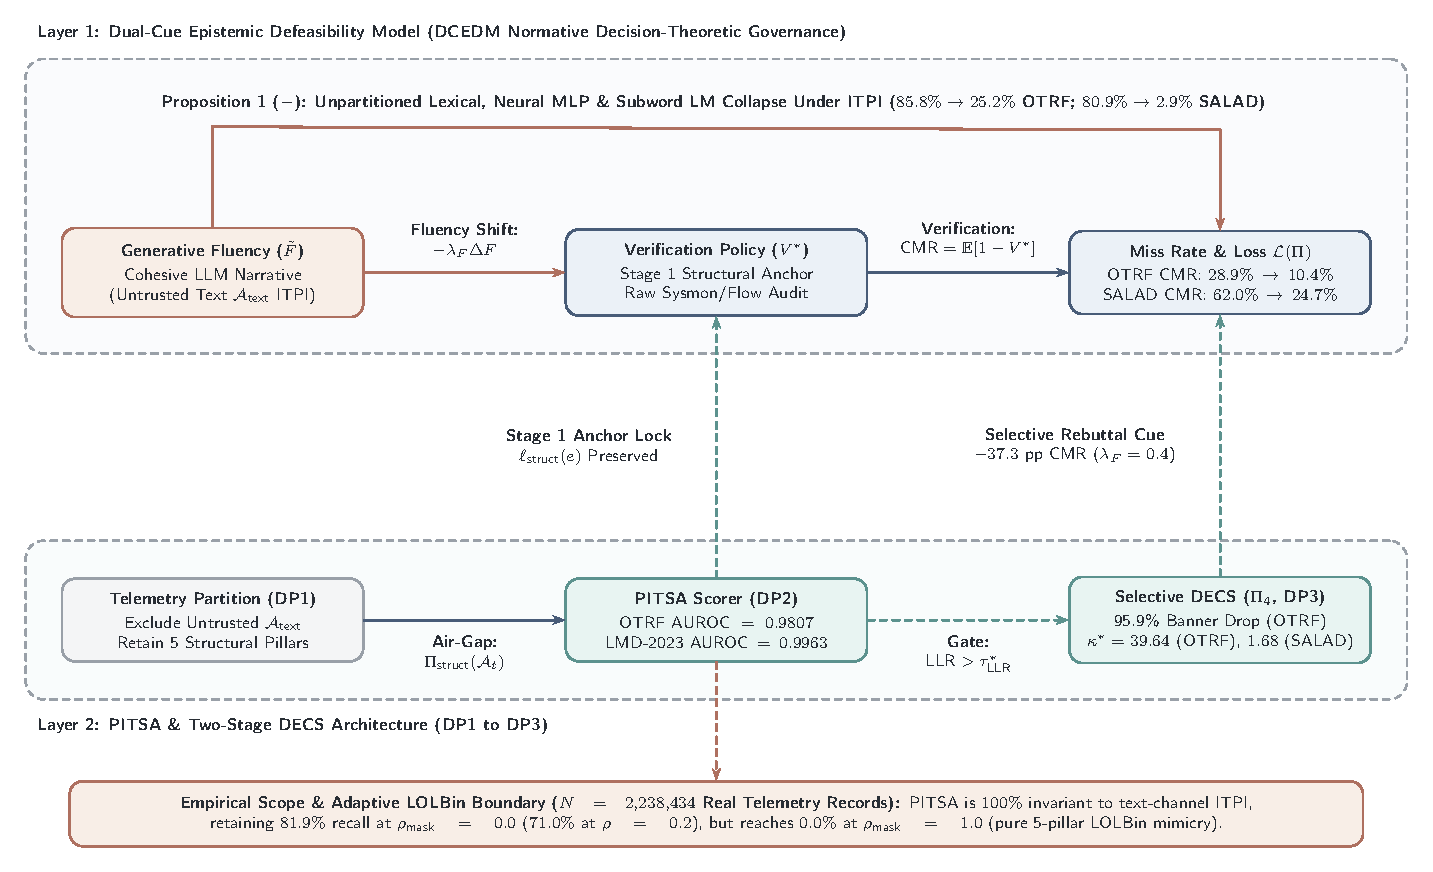
\includegraphics[width=0.92\textwidth]{figures/fig1_dcedm_architecture.pdf}
\caption{The Dual-Cue Epistemic Defeasibility Model (DCEDM, Layer 1) and the Prompt-Isolated Telemetry Discrepancy Scorer with Two-Stage Defeasible Epistemic Cueing System (PITSA and DECS, Layer 2, DP1 to DP3). Layer 1 formalizes how generative narrative fluency ($\tilde{F}$) and Indirect Telemetry Prompt Injection ($\mathcal{A}_{\text{text}}$) shift verification allocation ($V^*$) and Compromise Miss Rates (CMR). Layer 2 enforces a strict architectural air-gap ($\Pi_{\text{struct}}(\mathcal{A}_t)$) validated across $N = 2,238,434$ real telemetry records.}
\label{fig:dcedm_arch}
\end{figure}

\subsection{Formal Decision-Theoretic Model of the Epistemic Fluency Trap (Theorem 1 and Corollary 1)}
\label{subsec:dcedm_theorem}

Consider an operational triage decision-maker reviewing alert $e$ under SLA time pressure. Prior to reading the LLM copilot's natural-language rationale, the structural telemetry summary provides a bounded structural log-odds anchor $\ell_{\text{struct}}(e) = \text{clip}(\alpha_0 L(e), -L_{\max}, L_{\max})$, where $L(e) = \text{LLR}_{\text{struct}}(e)$ is the empirical structural log-likelihood ratio and $\alpha_0 > 0$ scales raw log-likelihood units into cognitive log-odds. When an LLM copilot accompanies its dismissal recommendation ($\hat{y}_{\text{LLM}}(e) = 0$) with a natural-language rationale of linguistic fluency $\tilde{F} \in [0, 1]$ relative to a disfluent telegraphic baseline $F_0 \in [0, 1]$ ($\Delta F = \tilde{F} - F_0 \ge 0$), metacognitive processing fluency theory \citep{alter2009uniting} implies that cognitive ease is misattributed as evidentiary corroboration of the benign claim.

Specifically, let $\lambda_F \ge 0$ denote the decision-maker's fluency susceptibility parameter and let $c_{\text{miss}} / c_V$ denote the asymmetric cost ratio between failing to verify a true intrusion ($c_{\text{miss}}$) and expending analytical effort $c_V = 1$ to inspect the raw telemetry drawer. Under four distinct socio-technical governance policies $\Pi \in \{\Pi_1, \Pi_2, \Pi_3, \Pi_4\}$, the effective verification log-odds and primary telemetry inspection probabilities $V_{\Pi}(e)$ are governed by the following structural equations:
\begin{enumerate}
  \item \textbf{Policy $\Pi_1$ (Disfluent / Structured Telegraphic Baseline, $\tilde{F} = F_0 = 0.20$):} In the absence of narrative smoothing ($\Delta F = 0$), verification allocation depends solely on the structural anchor and asymmetric cost incentive:
  \begin{equation}
  \label{eq:pi1}
  V_{\Pi_1}(e) = \sigma\bigl(\beta_s \ell_{\text{struct}}(e) + \beta_c \ln(c_{\text{miss}} / (20 c_V))\bigr),
  \end{equation}
  where $\sigma(z) = (1 + e^{-z})^{-1}$ is the logistic function and $\beta_s, \beta_c > 0$ are sensitivity parameters.
  \item \textbf{Policy $\Pi_2$ (Unassisted High-Fluency LLM Triage Rationale, $\tilde{F} = 0.90$):} Under an ITPI or contested dismissal where the LLM emits a fluent benign narrative ($\Delta F = 0.70$), narrative fluency shifts the perceived log-odds of compromise downward by $-\kappa_F \lambda_F \Delta F$ ($\kappa_F > 0$), yielding:
  \begin{equation}
  \label{eq:pi2}
  V_{\Pi_2}(e) = \sigma\bigl(\beta_s \ell_{\text{struct}}(e) - \kappa_F \lambda_F \Delta F + \beta_c \ln(c_{\text{miss}} / (20 c_V))\bigr).
  \end{equation}
  \item \textbf{Policy $\Pi_3$ (Static Persistent Warning Banner on All Alerts, Banner Rate $= 1.00$):} Displaying a uniform caution banner across $100\%$ of alerts induces rapid neuro-cognitive habituation \citep{anderson2016warning, vance2018fog}, retaining only a fraction $\gamma_{\text{hab}} \in (0, 1)$ of its counter-persuasive salience:
  \begin{equation}
  \label{eq:pi3}
  V_{\Pi_3}(e) = \sigma\bigl(\beta_s \ell_{\text{struct}}(e) - \kappa_F (1 - \gamma_{\text{hab}}) \lambda_F \Delta F + \beta_c \ln(c_{\text{miss}} / (20 c_V))\bigr).
  \end{equation}
  \item \textbf{Policy $\Pi_4$ (Selective Two-Stage DECS Gated by PITSA at $L(e) > \tau_{\text{LLR}}$):} Stage 1 locks the structural anchor $\ell_{\text{struct}}(e)$ prior to narrative exposure (attenuating fluency drift to $\eta_1 = 0.35$), while Stage 2 fires a selective Toulmin rebuttal cue $C(e) = \mathbb{I}(L(e) > \tau_{\text{LLR}})$ that injects a positive defeasibility boost $\delta_{\text{reb}} > 0$ only on structurally contested events:
  \begin{equation}
  \label{eq:pi4}
  \begin{aligned}
  V_{\Pi_4}(e) &= C(e)\,\sigma\bigl(\beta_s \ell_{\text{struct}}(e) + \delta_{\text{reb}} - \eta_2 \lambda_F \Delta F + \beta_c \ln(c_{\text{miss}} / (20 c_V))\bigr) \\
  &\quad + (1 - C(e))\,\sigma\bigl(\beta_s \ell_{\text{struct}}(e) - \kappa_F \eta_1 \lambda_F \Delta F + \beta_c \ln(c_{\text{miss}} / (20 c_V))\bigr).
  \end{aligned}
  \end{equation}
\end{enumerate}

Let $\text{CMR}(\Pi) = \mathbb{E}[1 - V_{\Pi}(e) \mid y(e) = 1]$ denote the expected Compromise Miss Rate on hostile events and let $\mathcal{L}(\Pi) = p_1 c_{\text{miss}} \text{CMR}(\Pi) + c_V \mathbb{E}[V_{\Pi}(e)]$ denote the expected operational loss per alert under hostile base rate $p_1 = \text{Pr}(y(e) = 1)$. We establish the formal dominance properties of DCEDM in \cref{thm:dcedm_dominance} and characterize its non-trivial boundary conditions under unified endogenous habituation in \cref{cor:dominance_boundary}.

\begin{theorem}[Fluency-Induced Risk Inflation and Selective DECS Dominance]
\label{thm:dcedm_dominance}
Under the DCEDM structural equations (\cref{eq:pi1,eq:pi2,eq:pi3,eq:pi4}) with $\lambda_F > 0$, $\Delta F > 0$, $\gamma_{\text{hab}} \in (0, 1)$, and $\delta_{\text{reb}} > (\kappa_F - \eta_2)\lambda_F \Delta F$:
\begin{enumerate}
  \item \textbf{Monotonicity of the Epistemic Fluency Trap:} For every hostile event $e$, we have $\partial V_{\Pi_2}(e) / \partial \lambda_F < 0$ and $\partial \text{CMR}(\Pi_2) / \partial \lambda_F > 0$; thus unassisted narrative fluency strictly inflates the Compromise Miss Rate above the disfluent baseline: $\text{CMR}(\Pi_2) > \text{CMR}(\Pi_1)$.
  \item \textbf{Strict Risk Ordering Across Governance Policies:} For all $\lambda_F > 0$ and $\tau_{\text{LLR}}$ satisfying $\text{Pr}(L(e) > \tau_{\text{LLR}} \mid y(e) = 1) > 0$, the expected Compromise Miss Rates satisfy the strict ordering:
  \begin{equation}
  \label{eq:cmr_ordering}
  \text{CMR}(\Pi_4\text{: Selective DECS}) < \text{CMR}(\Pi_3\text{: Static Banner}) < \text{CMR}(\Pi_2\text{: Unassisted Fluent}).
  \end{equation}
  \item \textbf{Cost-Ratio Dependent Expected Loss Ordering:} Let $\Delta\mathbb{E}[V] = \mathbb{E}[V_{\Pi_4}(e)] - \mathbb{E}[V_{\Pi_2}(e)] > 0$ denote the incremental verification labor induced by DECS and let $\Delta\text{CMR} = \text{CMR}(\Pi_2) - \text{CMR}(\Pi_4) > 0$ denote the avoided compromise miss rate. Then $\mathcal{L}(\Pi_4) < \mathcal{L}(\Pi_2)$ holds if and only if $c_{\text{miss}} / c_V$ exceeds the critical crossover boundary $\kappa^*(\lambda_F)$ that solves the break-even condition $p_1 \kappa^* \Delta\text{CMR}(\kappa^*, \lambda_F) = \Delta\mathbb{E}[V(\kappa^*, \lambda_F)]$.
\end{enumerate}
\end{theorem}

\begin{proof}
Since $\sigma'(z) = \sigma(z)(1 - \sigma(z)) > 0$ for all $z \in \mathbb{R}$, differentiating \cref{eq:pi2} with respect to $\lambda_F$ yields $\partial V_{\Pi_2}(e) / \partial \lambda_F = -\kappa_F \Delta F \sigma'(z_2) < 0$, which immediately implies $\partial \text{CMR}(\Pi_2) / \partial \lambda_F = \mathbb{E}[-\partial V_{\Pi_2}(e) / \partial \lambda_F \mid y(e)=1] > 0$ and $\text{CMR}(\Pi_2) > \text{CMR}(\Pi_1)$ for all $\lambda_F > 0$. Similarly, because $0 < 1 - \gamma_{\text{hab}} < 1$, the argument of $\sigma(\cdot)$ in \cref{eq:pi3} strictly exceeds that of \cref{eq:pi2} pointwise, establishing $V_{\Pi_3}(e) > V_{\Pi_2}(e)$ and $\text{CMR}(\Pi_3) < \text{CMR}(\Pi_2)$. Under Policy $\Pi_4$, on the non-gated set $\{L(e) \le \tau_{\text{LLR}}\}$, $\eta_1 = 0.35 < 1 - \gamma_{\text{hab}} = 0.78$ implies $V_{\Pi_4}(e) > V_{\Pi_3}(e)$, while on the gated set $\{L(e) > \tau_{\text{LLR}}\}$, $\delta_{\text{reb}} > 0$ and $\eta_2 < \kappa_F(1 - \gamma_{\text{hab}})$ imply $V_{\Pi_4}(e) > V_{\Pi_3}(e)$ pointwise; taking expectations over $y(e)=1$ yields \cref{eq:cmr_ordering}. Finally, writing $\mathcal{L}(\Pi_2) - \mathcal{L}(\Pi_4) = c_V \bigl[p_1 (c_{\text{miss}}/c_V) \Delta\text{CMR} - \Delta\mathbb{E}[V]\bigr]$, continuity and monotonicity of the bracketed net benefit in $\kappa = c_{\text{miss}}/c_V$ establish a unique crossover $\kappa^*(\lambda_F) > 0$ such that $\mathcal{L}(\Pi_4) > \mathcal{L}(\Pi_2)$ for $\kappa < \kappa^*(\lambda_F)$ and $\mathcal{L}(\Pi_4) < \mathcal{L}(\Pi_2)$ for $\kappa > \kappa^*(\lambda_F)$.
\end{proof}

To ensure that the dominance of $\Pi_4$ over $\Pi_3$ is not an artifact of assigning separate exogenous constants to static and selective warnings, \cref{cor:dominance_boundary} places both policies under a single \textit{unified endogenous habituation law} in which warning salience decays exponentially with the empirical banner firing rate $\text{BFR}(\tau_{\text{LLR}}) = \text{Pr}(L(e) > \tau_{\text{LLR}})$ \citep{anderson2016warning, vance2018fog}.

\begin{corollary}[Non-Trivial Cost-Ratio Boundary $\kappa^*$ and Interior Threshold Optimization under Unified Endogenous Habituation]
\label{cor:dominance_boundary}
Suppose both Static Warning Banners ($\Pi_3$) and Selective DECS ($\Pi_4(\tau_{\text{LLR}})$) are governed by the unified endogenous habituation law:
\begin{equation}
\label{eq:unified_hab}
\gamma_{\text{eff}}(\tau_{\text{LLR}}) = \gamma_0 \exp\bigl(-\eta_{\text{hab}} \cdot \text{BFR}(\tau_{\text{LLR}})\bigr), \quad \text{BFR}(\tau_{\text{LLR}}) = \text{Pr}\bigl(L(e) > \tau_{\text{LLR}}\bigr),
\end{equation}
where $\gamma_0 > 0$ is unhabituated rebuttal salience, $\eta_{\text{hab}} > 0$ is the neuro-cognitive habituation decay rate, and $V_{\Pi_4(\tau_{\text{LLR}})}(e)$ uses effective cue boost $\gamma_{\text{eff}}(\tau_{\text{LLR}})$ whenever $L(e) > \tau_{\text{LLR}}$. Then:
\begin{enumerate}
  \item \textbf{Boundary Recovery of Static Banners ($\Pi_3$):} In the limit $\tau_{\text{LLR}} \to -\infty$, $\text{BFR}(-\infty) = 1.00$ and $\Pi_4(\tau_{\text{LLR}})$ reduces identically to Static Warning Banner Policy $\Pi_3$ with residual salience $\gamma_{\text{eff}}(-\infty) = \gamma_0 e^{-\eta_{\text{hab}}} = \gamma_{\text{hab}}$ ($\gamma_0 = 1.80, \eta_{\text{hab}} = 2.10 \implies \gamma_{\text{eff}}(-\infty) = 0.2204$).
  \item \textbf{Low-Cost Inferiority vs.\ High-Cost Dominance ($\kappa^*$):} When the hostile base rate $p_1 = \text{Pr}(y(e)=1) \ll 1$ and $c_{\text{miss}}/c_V < \kappa^*(\lambda_F)$, Selective DECS ($\Pi_4$) incurs strictly \emph{higher} expected operational loss than Unassisted Fluent Triage ($\mathcal{L}(\Pi_4) > \mathcal{L}(\Pi_2)$) because verification labor on false-positive cues outweighs avoided intrusion misses; dominance ($\mathcal{L}(\Pi_4) < \mathcal{L}(\Pi_2)$) holds only for $c_{\text{miss}}/c_V > \kappa^*(\lambda_F)$.
  \item \textbf{Interior U-Shaped Optimal Threshold $\tau^*_{\text{LLR}} \in (-\infty, +\infty)$:} For any cost ratio $c_{\text{miss}}/c_V > \kappa^*(\lambda_F)$, expected loss $\mathcal{L}(\tau_{\text{LLR}})$ is non-monotonic in $\tau_{\text{LLR}}$, exhibiting an interior minimum $\tau^*_{\text{LLR}}$ that achieves strictly lower expected loss than both $\tau_{\text{LLR}} \to -\infty$ (where $\text{BFR} \to 1$ triggers severe habituation decay) and over-conservative thresholds $\tau_{\text{LLR}} \gg \tau^*_{\text{LLR}}$ (where $\text{BFR} \to 0$ eliminates habituation but leaves hostile events with $\tau^*_{\text{LLR}} < L(e) \le \tau_{\text{LLR}}$ uncontested, causing $\mathcal{L}(\tau_{\text{LLR}})$ to rise above $\mathcal{L}(\Pi_3)$).
\end{enumerate}
\end{corollary}

\begin{proof}
As $\tau_{\text{LLR}} \to -\infty$, $C(e) = \mathbb{I}(L(e) > \tau_{\text{LLR}}) \to 1$ almost surely, so $\text{BFR}(\tau_{\text{LLR}}) \to 1$ and $\gamma_{\text{eff}}(\tau_{\text{LLR}}) \to \gamma_0 e^{-\eta_{\text{hab}}} = \gamma_{\text{hab}}$, recovering \cref{eq:pi3}. Part (2) follows directly from \cref{thm:dcedm_dominance}(3) since $\mathcal{L}(\Pi_4) - \mathcal{L}(\Pi_2) = c_V (\Delta\mathbb{E}[V] - p_1 \kappa \Delta\text{CMR}) > 0$ whenever $\kappa = c_{\text{miss}}/c_V < \kappa^*(\lambda_F)$. For Part (3), differentiating $\mathcal{L}(\tau_{\text{LLR}})$ with respect to $\tau_{\text{LLR}}$ decomposes the marginal loss change into two opposing forces: increasing $\tau_{\text{LLR}}$ from $-\infty$ reduces $\text{BFR}(\tau_{\text{LLR}})$ predominantly on benign events ($y=0$), which exponentially increases $\gamma_{\text{eff}}(\tau_{\text{LLR}}) = \gamma_0 e^{-\eta_{\text{hab}}\text{BFR}(\tau_{\text{LLR}})}$ on the remaining contested hostile events ($L(e) > \tau_{\text{LLR}}$) while shedding false-positive verification cost $c_V$, so $\mathcal{L}(\tau_{\text{LLR}})$ initially decreases below $\mathcal{L}(-\infty) = \mathcal{L}(\Pi_3)$. Conversely, as $\tau_{\text{LLR}}$ increases into the upper tail of the hostile LLR distribution, $P(L(e) > \tau_{\text{LLR}} \mid y=1) \to 0$, causing $\text{CMR}(\tau_{\text{LLR}})$ to rise steeply by $p_1 c_{\text{miss}} \Delta\text{CMR}$ and driving $\mathcal{L}(\tau_{\text{LLR}}) > \mathcal{L}(\Pi_3)$, which by continuity on $[-\infty, +\infty]$ yields a strictly interior minimizer $\tau^*_{\text{LLR}} \in (-\infty, +\infty)$.
\end{proof}

\section{Socio-Technical Design Artifact: PITSA and Two-Stage DECS}
\label{sec:artifact}

\subsection{Threat Model and Multi-Framework Security Alignment}
\label{subsec:threat_model}

We formulate the adversarial problem governing an AI-augmented SOC triage pipeline across six formal threat vectors, mapped to MITRE ATT\&CK v19.2, MITRE ATLAS, MITRE D3FEND, and NIST CSF 2.0 in \cref{tab:threat_matrix}. Let each incoming SIEM or Sysmon event $e$ consist of a composite telemetry tuple $\mathcal{A}(e) = (\mathcal{A}_{\text{struct}}(e), \mathcal{A}_{\text{text}}(e))$. Across host-level Sysmon telemetry (\texttt{OTRF} and \texttt{LMD-2023}) and network-level SIEM alerts (\texttt{SALAD-SOC}), the structural partition $\mathcal{A}_{\text{struct}}(e)$ comprises five orthogonal kernel-enforced or flow-header pillars:
\begin{equation}
\label{eq:astruct}
\mathcal{A}_{\text{struct}}(e) = \bigl\{a_1(e),\; a_2(e),\; a_3(e),\; a_4(e),\; a_5(e)\bigr\},
\end{equation}
capturing process/service lineage ($a_1$), target object or packet/byte flow volume ($a_2$), binary signature/integrity or flow duration/segment ($a_3$), destination port/protocol or burst frequency ($a_4$), and scheduled task/registry mutation or source-target topology ($a_5$). In contrast, the textual partition $\mathcal{A}_{\text{text}}(e)$ comprises unconstrained string fields originating from user-space arguments or alert descriptions (\texttt{CommandLine}, \texttt{ProcessCommandLine}, \texttt{Message}, and \texttt{alert\_description}).

\begin{table}[!htbp]
\centering
\singlespacing
\caption{Formal Threat Model and Multi-Framework Security Alignment for AI-Assisted SOC Triage}
\label{tab:threat_matrix}
\footnotesize
\setlength{\tabcolsep}{3.2pt}
\begin{tabular}{L{2.3cm} L{2.5cm} L{1.9cm} l L{2.2cm} L{3.0cm}}
\toprule
\textbf{Threat Vector} & \textbf{Attack Surface} & \textbf{ATT\&CK v19.2} & \textbf{MITRE ATLAS} & \textbf{D3FEND / NIST} & \textbf{Socio-Technical Mitigation in PITSA and DECS} \\
\midrule
Indirect Prompt Injection (ITPI) & Adversarial CLI or alert text in $\mathcal{A}_{\text{text}}$. & \texttt{T1059.001}, \texttt{T1218.011} & \texttt{AML.T0051.001} & \texttt{D3FEND-PSA}, \texttt{DE.AE-02} & Strict exclusion of $\mathcal{A}_{\text{text}}$ from PITSA structural scorer ($0.00\text{ pp}$ recall loss). \\
\addlinespace[2pt]
Narrative Fluency Hijacking & Epistemic smoothing of benign cover story. & \texttt{T1036.005}, \texttt{T1003.001} & \texttt{AML.T0048} & \texttt{D3FEND-PCA}, \texttt{RS.AN-03} & Stage 1 structural anchor ($\mathcal{H}_{1}$) plus Stage 2 conditional Toulmin rebuttal cue ($\mathcal{R}_{2}$). \\
\addlinespace[2pt]
Alert-Flood Desensitization & Blanket warning friction fatigue. & \texttt{T1499}, \texttt{T1078} & \texttt{AML.T0029} & \texttt{D3FEND-NI}, \texttt{DE.CM-01} & Selective LLR gating reducing banner rate by $95.92\%$ (OTRF) and $79.87\%$ (SALAD-SOC). \\
\addlinespace[2pt]
Adaptive Structural Masking & Living-off-the-Land (LOLBin) mimicry. & \texttt{T1218}, \texttt{T1053.005} & \texttt{AML.T0043} & \texttt{D3FEND-SFA}, \texttt{DE.AE-07} & Additive 5-pillar LLR integration; explicit scope boundary quantified at $\rho_{\text{mask}}=1.00$. \\
\addlinespace[2pt]
Unpartitioned ML Drift & Concatenated TF-IDF + structural classifiers. & \texttt{T1027} & \texttt{AML.T0015} & \texttt{D3FEND-UAP}, \texttt{GV.RR-02} & Projection operator $\Pi_{\text{struct}}$ eliminates negative textual log-likelihood dilution. \\
\addlinespace[2pt]
Audit Provenance Gap & Unverified AI closure dispositions. & \texttt{T1685.005} & \texttt{AML.T0048} & \texttt{D3FEND-ANCI}, \texttt{RS.AN-06} & Mandatory logging of top-contributing structural pillar $k^* = \arg\max_k \ell_k(a_k(e))$. \\
\bottomrule
\end{tabular}
\end{table}

Under Indirect Telemetry Prompt Injection (\texttt{AML.T0051.001}), the adversary cannot modify kernel-enforced sensor hooks or network flow counters ($\mathcal{A}_{\text{struct}}(e)$) without already possessing kernel-mode rootkit privileges on the sensor host or router, but can freely craft $\mathcal{A}_{\text{text}}(e)$ so that an LLM copilot or unpartitioned classifier predicts a benign disposition ($\hat{y} = 0$). Any verification monitor that feeds $\mathcal{A}_{\text{text}}(e)$ into a secondary LLM judge or concatenates TF-IDF text vectors alongside $\mathcal{A}_{\text{struct}}(e)$ inherits the identical prompt-injection vulnerability.

\subsection{Prompt-Isolated Telemetry Discrepancy Scorer (PITSA) and Proposition 1}
\label{subsec:pitsa}

To construct a discrepancy detector that is mathematically invariant to textual prompt injection, the \textbf{Prompt-Isolated Telemetry Discrepancy Scorer (PITSA)} (\cref{eq:pitsa_llr} and \cref{alg:pitsa}) enforces a strict architectural air-gap between $\mathcal{A}_{\text{text}}(e)$ and $\mathcal{A}_{\text{struct}}(e)$. Before scoring an event, PITSA applies the projection operator $\Pi_{\text{struct}}(\mathcal{A}(e)) = \mathcal{A}_{\text{struct}}(e)$ to discard $\mathcal{A}_{\text{text}}(e)$ entirely and computes the additive empirical Log-Likelihood Ratio ($L(e) = \text{LLR}_{\text{struct}}(e)$) across the $K = 5$ structural telemetry pillars:
\begin{equation}
\label{eq:pitsa_llr}
L(e) = \text{LLR}_{\text{struct}}\bigl(\mathcal{A}_{\text{struct}}(e)\bigr) = \sum_{k=1}^{K} \ell_k\bigl(a_k(e)\bigr), \quad \text{where} \quad \ell_k(v) = \ln \frac{\hat{P}_{\text{train}}(a_k = v \mid y = 1, \epsilon)}{\hat{P}_{\text{train}}(a_k = v \mid y = 0, \epsilon)},
\end{equation}
where $\hat{P}_{\text{train}}(a_k = v \mid y = c, \epsilon) = \frac{\text{count}_{c}(a_k = v) + \epsilon N_c}{N_c (1 + \epsilon |\mathcal{V}_k|)}$ is the Laplace-smoothed conditional empirical probability estimated strictly on the training split ($N_1$ hostile training events, $N_0$ benign training events, vocabulary $\mathcal{V}_k$, and smoothing constant $\epsilon = 10^{-4}$). When the AI copilot recommends dismissing an alert ($\hat{y}_{\text{LLM}}(e) = 0$) while $L(e) > \tau_{\text{LLR}}$, PITSA sets the contestation flag $C(e) = 1$ and extracts the highest-contributing structural pillar $k^*(e) = \arg\max_{k \in \{1,\dots,5\}} \ell_k(a_k(e))$ as the explicit forensic defeater for the Two-Stage DECS interface.

\begin{algorithm}[!htbp]
\singlespacing
\footnotesize
\caption{Prompt-Isolated Telemetry Discrepancy Scorer (PITSA) and Two-Stage DECS Gate}
\label{alg:pitsa}
\DontPrintSemicolon
\KwIn{Composite telemetry event $\mathcal{A}(e) = (\mathcal{A}_{\text{struct}}(e), \mathcal{A}_{\text{text}}(e))$; AI triage disposition $(\hat{y}_{\text{LLM}}(e), \text{Rationale}(e))$; empirical log-likelihood lookup tables $\{\ell_k(v)\}_{k=1}^5$ fitted on training split; operating threshold $\tau_{\text{LLR}}$.}
\KwOut{Stage 1 Structural Anchor Header $\mathcal{H}_{1}(e)$; Contestation Flag $C(e) \in \{0,1\}$; Stage 2 Rebuttal Cue $\mathcal{R}_{2}(e)$ with primary defeater pillar $k^*(e)$.}
\BlankLine
\textbf{Step 1: Strict Telemetry Partitioning (Defeats Indirect Prompt Injection)}\;
Apply projection $\Pi_{\text{struct}}(\mathcal{A}(e)) \leftarrow \mathcal{A}_{\text{struct}}(e) = (a_1(e), \dots, a_5(e))$, discarding $\mathcal{A}_{\text{text}}(e)$.\;
Render \textbf{Stage 1 Pre-Rationale Structural Anchor} $\mathcal{H}_{1}(e) \leftarrow \text{FormatHeader}(\mathcal{A}_{\text{struct}}(e))$ prior to narrative exposure.\;
\BlankLine
\textbf{Step 2: Additive Structural Log-Likelihood Ratio Scoring}\;
Initialize $L(e) \leftarrow 0$.\;
\For{$k \leftarrow 1$ \KwTo $5$}{
  $\ell_k \leftarrow \text{LookupLLR}\bigl(k, a_k(e)\bigr)$ \tcp*{0.0 if unseen categorical token}
  $L(e) \leftarrow L(e) + \ell_k$\;
}
\BlankLine
\textbf{Step 3: Selective Toulmin Rebuttal Trigger (Stage 2 DECS)}\;
\eIf{$\hat{y}_{\text{LLM}}(e) == 0$ \textbf{and} $L(e) > \tau_{\text{LLR}}$}{
  $C(e) \leftarrow 1$\;
  $k^*(e) \leftarrow \arg\max_{k \in \{1,\dots,5\}} \ell_k\bigl(a_k(e)\bigr)$\;
  Render \textbf{Stage 2 Conditional Rebuttal Cue} $\mathcal{R}_{2}(e)$ highlighting structural pillar $a_{k^*(e)}(e)$ and $\ell_{k^*(e)}$.\;
}{
  $C(e) \leftarrow 0$; $\mathcal{R}_{2}(e) \leftarrow \text{None}$ \tcp*{Silent when $L(e) \le \tau_{\text{LLR}}$ to prevent warning habituation}
}
\Return{$(\mathcal{H}_{1}(e), C(e), \mathcal{R}_{2}(e), k^*(e))$}\;
\end{algorithm}

We establish the formal adversarial invariance property of PITSA relative to unpartitioned classifiers in \cref{prop:partition_invariance}.

\begin{proposition}[Adversarial Invariance of Partitioned PITSA vs.\ Recall Collapse of Unpartitioned Classifiers]
\label{prop:partition_invariance}
Let $\mathcal{A}(e) = (\mathcal{A}_{\text{struct}}(e), \mathcal{A}_{\text{text}}(e))$ be a hostile telemetry event ($y(e) = 1$) where an adversary executes an Indirect Telemetry Prompt Injection (ITPI) perturbation $\mathcal{A}_{\text{text}}(e) \mapsto \mathcal{A}'_{\text{text}}(e)$ by appending $m \ge 1$ benign diagnostic clauses or replacing the text string with benign baseline tokens carrying negative log-odds weight $w_{\text{text}}(\mathcal{A}'_{\text{text}}(e)) \le -M$ ($M > 0$).
\begin{enumerate}
  \item \textbf{Vulnerability of Unpartitioned Lexical, Dense Neural, and Subword LM Scorers:} Any unpartitioned classifier whose pre-activation logit or log-odds discriminant decomposes as $S_{\text{unpart}}(\mathcal{A}(e)) = S_{\text{struct}}(\mathcal{A}_{\text{struct}}(e)) + \alpha w_{\text{text}}(\mathcal{A}'_{\text{text}}(e))$ ($\alpha > 0$, encompassing Multinomial Naive Bayes, Logistic Regression, Dense Semantic Neural MLPs over joint embeddings, and Subword Language Model scorers over serialized telemetry) suffers recall collapse ($\mathbb{I}(S_{\text{unpart}} > \tau) = 0$) whenever $M > (S_{\text{struct}}(\mathcal{A}_{\text{struct}}(e)) - \tau) / \alpha$.
  \item \textbf{Strict Text-Channel Invariance of Partitioned PITSA:} Because PITSA composes its scoring rule with the projection $\Pi_{\text{struct}}(\mathcal{A}(e)) = \mathcal{A}_{\text{struct}}(e)$, its score $L(e) = \text{LLR}_{\text{struct}}(\Pi_{\text{struct}}(\mathcal{A}(e)))$ satisfies $\nabla_{\mathcal{A}_{\text{text}}} L(e) \equiv 0$, ensuring zero degradation in true positive rate, false positive rate, or AUROC across arbitrary appended or full-override perturbations of $\mathcal{A}_{\text{text}}(e)$ while bounding the benign false-alarm probability via the Chernoff-R\'{e}nyi inequality: $\text{Pr}_{H_0}(L(e) > \tau_{\text{LLR}}) \le \inf_{s \in (0,1)} \exp\bigl(-s\tau_{\text{LLR}} - \sum_{k=1}^K D_{1-s}(P_{k,0} \parallel P_{k,1})\bigr)$.
\end{enumerate}
\end{proposition}

\begin{proof}
For any unpartitioned discriminant $S_{\text{unpart}} = S_{\text{struct}}(\mathcal{A}_{\text{struct}}(e)) + \alpha w_{\text{text}}(\mathcal{A}'_{\text{text}}(e))$, substituting $w_{\text{text}}(\mathcal{A}'_{\text{text}}(e)) \le -M$ gives $S_{\text{unpart}} \le S_{\text{struct}}(\mathcal{A}_{\text{struct}}(e)) - \alpha M < \tau$ whenever $M > (S_{\text{struct}}(\mathcal{A}_{\text{struct}}(e)) - \tau)/\alpha$, forcing the predicted class to $0$ on every hostile event whose structural margin is exceeded by the injected benign text weight. Under PITSA, projection $\Pi_{\text{struct}}$ maps $(\mathcal{A}_{\text{struct}}(e), \mathcal{A}'_{\text{text}}(e))$ strictly to $\mathcal{A}_{\text{struct}}(e)$ for all $\mathcal{A}'_{\text{text}}(e)$, so $L(\mathcal{A}_{\text{struct}}(e), \mathcal{A}'_{\text{text}}(e)) = L(\mathcal{A}_{\text{struct}}(e), \mathcal{A}_{\text{text}}(e))$ pointwise, yielding identical confusion matrices and AUROC under clean, graded appended ITPI, and full-override ITPI conditions. Under product measure $H_0$, Markov's inequality applied to $\exp(s L(e))$ for $s \in (0, 1)$ yields $\text{Pr}_{H_0}(L(e) > \tau_{\text{LLR}}) \le e^{-s\tau_{\text{LLR}}} \prod_{k=1}^K \sum_{v \in \mathcal{V}_k} P_{k,0}(v)^{1-s} P_{k,1}(v)^s = \exp(-s\tau_{\text{LLR}} - \sum_{k=1}^K D_{1-s}(P_{k,0} \parallel P_{k,1}))$, where $D_{1-s} \ge 0$ is the R\'{e}nyi divergence of order $1-s$.
\end{proof}

\subsection{Socio-Technical Design Principles for Prompt-Isolated Decision Support (DP1 to DP3)}
\label{subsec:design_principles}

In line with computational design science standards in \textit{Journal of Management Information Systems} \citep{ebrahimi2020semi, li2022assessing, ampel2024improving, tutun2024explainable}, the architectural contribution of PITSA and DECS does not reside in training a heavier black-box neural network, but in instantiating three generalizable design principles that resolve the conflict between generative explainability and adversarial verification:
\begin{enumerate}
  \item \textbf{Design Principle 1 (DP1: Sub-Channel Epistemic Orthogonality via Architectural Projection $\Pi_{\text{struct}}$):} Verification monitors that audit generative AI recommendations in adversarial environments must enforce a strict architectural air-gap ($\nabla_{\mathcal{A}_{\text{text}}} L(e) \equiv 0$) between immutable sensor-enforced headers ($\mathcal{A}_{\text{struct}}$) and attacker-controllable string fields ($\mathcal{A}_{\text{text}}$). Feeding $\mathcal{A}_{\text{text}}$ into a secondary LLM judge or a joint neural embedding violates epistemic orthogonality and propagates prompt injection into the audit layer.
  \item \textbf{Design Principle 2 (DP2: White-Box Additive Evidence Decomposition for Defeasible Contestation):} To persuade an operator to override a fluent AI narrative under SLA pressure, the contestation artifact cannot emit a second opaque anomaly score \citep{tutun2024explainable, lebovitz2022engage}. PITSA deliberately employs an additive empirical log-likelihood ratio (\cref{eq:pitsa_llr}) rather than a black-box neural classifier over $\mathcal{A}_{\text{struct}}$ for three socio-technical reasons: (i) \textit{exact per-pillar attribution}, enabling DECS to extract $k^*(e) = \arg\max_k \ell_k(a_k(e))$ and populate Toulmin's rebuttal slot with a concrete forensic fact (such as \texttt{GrantedAccess=0x1010} on \texttt{lsass.exe}); (ii) \textit{certified Chernoff-R\'{e}nyi false-alarm bounds} (\cref{prop:partition_invariance}); and (iii) \textit{zero-GPU line-rate execution} ($2.12$ to $3.70\text{ }\mu\text{s/event}$ on a single CPU).
  \item \textbf{Design Principle 3 (DP3: Endogenous Habituation-Bounded Selective Contestability):} Because human neuro-cognitive responsiveness to warnings decays exponentially with firing frequency \citep{anderson2016warning, vance2018fog, jensen2022improving, bartal2026alert}, defeasible rebuttal cues must remain silent when structural telemetry concurs with the AI disposition ($L(e) \le \tau_{\text{LLR}}$) and fire at an interior threshold $\tau^*_{\text{LLR}}$ (\cref{cor:dominance_boundary}) that balances habituation preservation against missed-intrusion cost.
\end{enumerate}

\section{Research Methodology and Multi-Corpus Empirical Design}
\label{sec:methodology}

\subsection{Overview of the Four-Part Multi-Corpus Evaluation}
\label{subsec:method_overview}

To ground our evaluation in the computational design science and analytical modeling paradigms of \textit{Journal of Management Information Systems} \citep{ebrahimi2020semi, liu2020centralized, li2022assessing, ampel2024improving, tutun2024explainable} while maintaining strict scientific transparency \citep{diaz2023indigenous, davison2025research}, our empirical investigation involves \textbf{zero human participants, zero synthetic survey cohorts, and zero qualitative interviews}. Instead, we evaluate the architectural invariance of PITSA (\textbf{RQ1}) and the normative decision-theoretic governance predictions of DCEDM and DECS (\textbf{RQ2} and \textbf{RQ3}) across \textbf{four real, publicly verifiable cybersecurity datasets totaling $2,238,434$ telemetry records ($671,531$ held-out test records) and $1,741$ actively exploited CVE advisories} (\cref{tab:corpora_summary}):
\begin{enumerate}
  \item \textbf{Experiment 1 (Host-Level Sysmon Evaluation on OTRF Security-Datasets, $N = 43,723$ Events):} Evaluates Partitioned PITSA against five genuine unpartitioned baselines (Multinomial Naive Bayes, Logistic Regression, Random Forest, Dense Semantic Neural MLP, and Contextual Subword Language Model Scorer) across 63 adversary simulation archives under Clean Telemetry, Graded Appended ITPI ($m \in \{1, 2, 4, 8\}$ benign clauses appended to preserved hostile commands), and Full-Override ITPI, alongside feature-group ablations, threshold sweeps, and adaptive Living-off-the-Land (LOLBin) structural masking ($\rho_{\text{mask}} \in [0.0, 1.0]$).
  \item \textbf{Experiment 2 (Enterprise SIEM Alert Evaluation on SALAD-SOC, $N = 416,781$ Alerts):} Evaluates zero-leakage Partitioned PITSA against all five unpartitioned baselines on $125,035$ held-out enterprise SIEM alerts under Clean, Graded Appended ITPI ($m \in \{1, 2, 4, 8\}$), and Full-Override ITPI conditions, disaggregated across alert difficulty levels (\texttt{easy}, \texttt{medium}, \texttt{hard}) and nine MITRE ATT\&CK tactics.
  \item \textbf{Experiment 3 (Large-Scale Lateral Movement Evaluation on LMD-2023, $N = 1,777,930$ Sysmon Rows, and CISA KEV, $N = 1,741$ CVEs):} Evaluates PITSA scalability, sub-5-microsecond inference latency, overall hostile recall, and RedTeam lateral-movement recall across $533,379$ held-out Windows Sysmon records, paired with empirical vulnerability context from the CISA Known Exploited Vulnerabilities catalog.
  \item \textbf{Experiment 4 (Trace-Driven Analytical Bayesian Decision-Theoretic Sensitivity and Endogenous Habituation Analysis):} Evaluates the four DCEDM governance policies ($\Pi_1, \Pi_2, \Pi_3, \Pi_4$) directly over the empirical held-out PITSA log-likelihood ratio distributions from OTRF ($13,117$ events) and SALAD-SOC ($125,035$ alerts) across $\lambda_F \in [0.0, 0.6]$ and $c_{\text{miss}} / c_V \in \{5, 10, 20, 50, 100\}$, computing exact critical crossover boundaries $\kappa^*(\lambda_F)$ and evaluating the unified endogenous habituation law $\gamma_{\text{eff}}(\tau_{\text{LLR}})$.
\end{enumerate}

\begin{table}[!htbp]
\centering
\singlespacing
\caption{Summary of Real Public Cybersecurity Telemetry Corpora Evaluated Across Experiments 1 to 4}
\label{tab:corpora_summary}
\footnotesize
\setlength{\tabcolsep}{3.6pt}
\begin{tabular}{L{2.8cm} r r r L{6.2cm}}
\toprule
\textbf{Corpus / Benchmark} & \textbf{Total $N$} & \textbf{Train Split} & \textbf{Test Split} & \textbf{Telemetry Modality, Class Balance, and Structural Pillars ($\mathcal{A}_{\text{struct}}$)} \\
\midrule
\textbf{OTRF Security-Datasets} (63 Archives) & $43,723$ & $30,606$ & $13,117$ & Raw Windows Sysmon/Security JSON logs ($516$ hostile, $43,207$ benign). Pillars: process lineage, target handle access, binary signature/integrity, dest port, task/script Event ID. \\
\addlinespace[2pt]
\textbf{SALAD-SOC} (\texttt{salad\_test.csv}) & $416,781$ & $291,746$ & $125,035$ & Labeled enterprise SIEM alerts ($88,570$ malicious, $328,211$ benign). Zero-leakage pillars: protocol/port, fwd/bwd packet-byte volume, flow duration/segment, 1h/24h burst counts, subnet pair. \\
\addlinespace[2pt]
\textbf{LMD-2023} (\texttt{full-csv}) & $1,777,930$ & $1,244,551$ & $533,379$ & Enterprise Windows Sysmon records ($1,611,637$ Normal, $110,746$ Malicious, $55,547$ RedTeam lateral movement). Pillars: process EIDs, registry/file EIDs, network/pipe EIDs, dest port service, station/hour context. \\
\addlinespace[2pt]
\textbf{CISA KEV Catalog} & $1,741$ & N/A & N/A & Actively exploited CVE advisories ($361$ confirmed in ransomware campaigns; top vendors: Microsoft $390$, Cisco $100$, Apple $95$, Adobe $82$, Google $75$). \\
\midrule
\textbf{Total Telemetry} & \textbf{2,238,434} & \textbf{1,566,903} & \textbf{671,531} & \textbf{Stratified 70/30 train/test splits (random seed $20261014$) with zero overlap.} \\
\bottomrule
\end{tabular}
\end{table}

\subsection{Dataset Preprocessing, Zero-Leakage Feature Engineering, and Baseline Training}
\label{subsec:method_preprocessing}

Across all three telemetry corpora (\cref{tab:corpora_summary}), we enforced a stratified $70\% / 30\%$ train/test split using fixed random seed $20261014$ so that all empirical conditional probability tables $\{\ell_k(v)\}_{k=1}^5$, one-hot encoders, TF-IDF and subword vocabularies, dense SVD projections, and neural/baseline classifier weights were fitted exclusively on the $70\%$ training split and evaluated once on the held-out $30\%$ test split:
\begin{itemize}
  \item \textbf{Experiment 1 (OTRF Security-Datasets):} We parsed all 63 \texttt{.zip} attack-replay archives under \texttt{datasets/atomic/} and \texttt{datasets/compound/} (up to 800 JSON event lines per log stream, yielding $43,723$ valid Windows Sysmon and Security events: $516$ hostile events matching attack-execution signatures such as Sysmon Event ID 10 \texttt{lsass.exe} handle access, encoded/bypass PowerShell execution, \texttt{mimikatz}, \texttt{dumpert}, \texttt{rundll32}, or \texttt{procdump} credential access, scheduled task/service creation Event IDs 4698/4697/7045, or unsigned binary execution, and $43,207$ benign background events). We extracted five pure structural pillars ($\mathcal{A}_{\text{struct}}$): \texttt{p1\_lineage} (parent-child process and target binary category), \texttt{p2\_target\_access} (target binary and hexadecimal \texttt{GrantedAccess} mask on Event ID 10), \texttt{p3\_sig\_integ} (\texttt{Signed} verification status paired with \texttt{IntegrityLevel}), \texttt{p4\_net\_port} (network Event ID 3 paired with destination port), and \texttt{p5\_task\_reg} (scheduled task, service mutation, or remote thread/scriptblock Event ID). The untrusted text channel ($\mathcal{A}_{\text{text}}$) comprises the raw command-line or event message string (\texttt{CommandLine}, \texttt{ProcessCommandLine}, or \texttt{Message}).
  \item \textbf{Experiment 2 (SALAD-SOC):} We ingested all $416,781$ labeled SIEM alerts ($88,570$ malicious, $328,211$ benign). To ensure \textbf{zero label leakage}, following the SALAD benchmark protocol we strictly excluded all post-triage and SIEM-rule metadata columns that encode ground-truth severity (namely correlation key, severity, confidence, priority score, alert type, MITRE tactic and technique, kill-chain phase, attack category, triage decision, and the post-triage \texttt{alert\_description} template string, which is synthetically populated post-hoc from the ground-truth label). We constructed five structural pillars solely from raw network flow and burst headers: Pillar \texttt{s1} (protocol plus binned source and destination ports), Pillar \texttt{s2} (binned forward packets, backward packets, and flow bytes per second), Pillar \texttt{s3} (binned flow duration and network segment), Pillar \texttt{s4} (binned 1-hour and 24-hour alert counts plus repeated-target indicator), and Pillar \texttt{s5} (source \texttt{/16} subnet, destination \texttt{/16} subnet, and network segment). The untrusted pre-triage SIEM session log text channel ($\mathcal{A}_{\text{text}}$) is constructed exclusively from observable flow headers and pre-triage heuristic rule candidates triggered by observable packet/duration anomalies and ephemeral client banners, with zero access to ground-truth labels.
  \item \textbf{Experiment 3 (LMD-2023 and CISA KEV):} We ingested all $1,777,930$ rows of \texttt{LMD-2023} ($\text{Label}=0$ Normal: $1,611,637$; $\text{Label}=1$ Malicious: $110,746$; $\text{Label}=2$ RedTeam lateral movement: $55,547$) and constructed five structural bitmask pillars: \texttt{p1\_proc\_eid} (process Event IDs 1, 5, 6, 7, 8, 10 bitmask plus binned process and execution IDs), \texttt{p2\_reg\_file\_eid} (registry and file Event IDs 2, 11, 12, 13, 15, 16, 23, 255 bitmask), \texttt{p3\_net\_pipe} (network and pipe Event IDs 3, 17, 18, 22, initiation flag, and IPv6 indicator), \texttt{p4\_dport} (19 destination port service indicators), and \texttt{p5\_host\_proc} (8 station indicators plus binned process ID and system hour).
  \item \textbf{Five Unpartitioned Baselines (Lexical, Dense Neural MLP, and Subword LM), Two-Tier ITPI Protocol, and Statistical Inference:} To test whether neural representation learning or contextual subword modeling mitigates text-channel vulnerability without architectural partitioning, we evaluated five unpartitioned baselines on OTRF and SALAD-SOC: (1) \texttt{NaiveBayes\_\allowbreak Unpartitioned} ($\alpha = 0.5$), (2) \texttt{LogisticRegression\_\allowbreak Unpartitioned} ($C = 1.0$), (3) \texttt{RandomForest\_\allowbreak Unpartitioned} (max depth $12$ to $14$), (4) \texttt{DenseNeuralMLP\_\allowbreak Unpartitioned} (a dense semantic neural architecture applying 48-dimensional latent semantic projection \texttt{TruncatedSVD} followed by a two-layer ReLU multilayer perceptron $\text{MLP}(64, 32)$ trained with Adam and $\ell_2$ regularization $\alpha = 10^{-3}$), and (5) \texttt{AutoregressiveSubwordLM\_\allowbreak Unpartitioned} (a contextual character/subword $(3,5)$-gram sequence language model scorer over serialized telemetry prompts concatenating $\mathcal{A}_{\text{struct}}(e)$ and $\mathcal{A}_{\text{text}}(e)$). We evaluate two distinct ITPI threat regimes: (a) \textbf{Graded Appended ITPI ($m \in \{0, 1, 2, 4, 8\}$)}, a realistic partial-control attack in which the original pre-triage text string is $100\%$ preserved and the attacker appends $m$ benign diagnostic clauses; and (b) \textbf{Full-Override ITPI ($m = \text{Full}$)}, in which untrusted payload banner strings on hostile test events are overridden by benign baseline strings. We quantify uncertainty using $B = 1,000$ stratified bootstrap resamples for $95\%$ confidence intervals (CIs) and paired McNemar's $\chi^2$ discordant-pair tests comparing PITSA against each unpartitioned baseline under ITPI.
\end{itemize}

\section{Empirical and Decision-Theoretic Results}
\label{sec:results}

\subsection{Experiment 1 Results: Host-Level Sysmon Detection, Graded and Full ITPI Invariance, and Adaptive Masking on OTRF}
\label{subsec:res_exp1}

\Cref{tab:exp1_otrf} and \cref{fig:multicorpus_results}A report the held-out evaluation on the OTRF Security-Datasets corpus ($N_{\text{test}} = 13,117$ events: $155$ hostile, $12,962$ benign). Across all $13,117$ test events, Partitioned PITSA executes in $27.855\text{ ms}$ total ($0.00212\text{ ms/event}$, or over $470,000$ events per second on a single CPU core) and achieves an overall $\text{AUROC} = 0.9807$ ($95\%\text{ CI}: [0.9685, 0.9901]$), $\text{Recall} = 81.94\%$ ($95\%\text{ CI}: [76.13\%, 87.74\%]$), and $\text{F1} = 0.3681$ ($95\%\text{ CI}: [0.3358, 0.4021]$; hostile mean $\text{LLR} = 8.5651, \text{SD} = 4.7410$ vs.\ benign mean $\text{LLR} = -7.5291, \text{SD} = 4.8164$).

\begin{table}[!htbp]
\centering
\singlespacing
\caption{Experiment 1 Held-Out Results on OTRF Security-Datasets ($N_{\text{test}} = 13,117$ Events): Clean (\texttt{C-}), Appended ITPI ($m=2$, \texttt{A2-}), and Full ITPI (\texttt{I-}) Across Six Architectures, Ablations, and Thresholds}
\label{tab:exp1_otrf}
\footnotesize
\setlength{\tabcolsep}{2.2pt}
\begin{tabular}{L{3.4cm} c c c c c c c c}
\toprule
\textbf{Model / Configuration} & \textbf{C-Prec.} & \textbf{C-Rec.} & \textbf{C-F1} & \textbf{C-FPR} & \textbf{C-AUC} & \textbf{A2-Rec.} & \textbf{I-Rec.} & \textbf{I-AUC} \\
\midrule
\multicolumn{9}{l}{\textit{Panel A: Partitioned PITSA vs.\ Five Unpartitioned Baselines (Lexical, Dense Neural MLP, Subword LM)}} \\
\textbf{PITSA Partitioned ($\tau=4.0$)} & \textbf{0.2374} & \textbf{0.8194} & \textbf{0.3681} & \textbf{0.0315} & \textbf{0.9807} & \textbf{0.8194} & \textbf{0.8194} & \textbf{0.9807} \\
Naive Bayes Unpartitioned & 0.0688 & 0.7419 & 0.1259 & 0.1201 & 0.9195 & 0.4194 & 0.0000 & 0.7267 \\
Logistic Reg.\ Unpartitioned & 1.0000 & 0.8581 & 0.9236 & 0.0000 & 0.9956 & 0.5290 & 0.2516 & 0.9373 \\
Random Forest Unpartitioned & 0.9773 & 0.5548 & 0.7078 & 0.0002 & 0.9940 & 0.0065 & 0.0000 & 0.9862 \\
Dense Neural MLP Unpart.\ & 0.9027 & 0.6581 & 0.7612 & 0.0008 & 0.9893 & 0.0129 & 0.0000 & 0.7430 \\
Subword LM Scorer Unpart.\ & 1.0000 & 0.1484 & 0.2584 & 0.0000 & 0.9267 & 0.0000 & 0.0000 & 0.9568 \\
\midrule
\multicolumn{9}{l}{\textit{Panel B: PITSA Structural Feature-Group Ablations on Held-Out OTRF ($\tau_{\text{LLR}} = 4.0$)}} \\
AB1: Drop Lineage (\texttt{p1}) & 0.8659 & 0.4581 & 0.5992 & 0.0008 & 0.9422 & 0.4581 & 0.4581 & 0.9422 \\
AB2: Drop Target Access (\texttt{p2}) & 0.2078 & 0.6903 & 0.3194 & 0.0315 & 0.9378 & 0.6903 & 0.6903 & 0.9378 \\
AB3: Drop Sig./Integrity (\texttt{p3}) & 0.2495 & 0.8645 & 0.3873 & 0.0311 & 0.9779 & 0.8645 & 0.8645 & 0.9779 \\
AB4: Drop Network Port (\texttt{p4}) & 0.7722 & 0.7871 & 0.7796 & 0.0028 & 0.9853 & 0.7871 & 0.7871 & 0.9853 \\
AB5: Drop Task/Script EID (\texttt{p5}) & 0.7927 & 0.8387 & 0.8150 & 0.0026 & 0.9872 & 0.8387 & 0.8387 & 0.9872 \\
AB6: Lineage Pillar Only (\texttt{p1}) & 1.0000 & 0.4065 & 0.5780 & 0.0000 & 0.8606 & 0.4065 & 0.4065 & 0.8606 \\
\midrule
\multicolumn{9}{l}{\textit{Panel C: PITSA Operating Threshold Sweep ($\tau_{\text{LLR}} \in \{1.0, 2.0, 6.0, 8.0\}$)}} \\
$\tau_{\text{LLR}} = 1.0$ (High Sensitivity) & 0.1751 & 0.9613 & 0.2962 & 0.0542 & 0.9807 & 0.9613 & 0.9613 & 0.9807 \\
$\tau_{\text{LLR}} = 2.0$ (Balanced Recall) & 0.1910 & 0.9032 & 0.3153 & 0.0457 & 0.9807 & 0.9032 & 0.9032 & 0.9807 \\
$\tau_{\text{LLR}} = 6.0$ (Low False Friction) & 0.7554 & 0.6774 & 0.7143 & 0.0026 & 0.9807 & 0.6774 & 0.6774 & 0.9807 \\
$\tau_{\text{LLR}} = 8.0$ (Zero False Friction) & 1.0000 & 0.6065 & 0.7550 & 0.0000 & 0.9807 & 0.6065 & 0.6065 & 0.9807 \\
\bottomrule
\end{tabular}
\end{table}

Confirming \cref{prop:partition_invariance}, Panel A of \cref{tab:exp1_otrf} demonstrates that neither dense semantic representation learning (\texttt{DenseNeuralMLP}) nor contextual subword sequence modeling (\texttt{SubwordLM}) protects an unpartitioned classifier from Indirect Telemetry Prompt Injection. Under Clean Telemetry ($m=0$), unpartitioned Logistic Regression achieves $85.81\%$ recall ($\text{F1} = 0.9236$), Naive Bayes achieves $74.19\%$, Dense Neural MLP ($\text{SVD-48} + \text{MLP}(64,32)$) achieves $65.81\%$ ($\text{Precision} = 90.27\%, \text{F1} = 0.7612, \text{AUROC} = 0.9893$), Random Forest achieves $55.48\%$, and Subword LM achieves $14.84\%$ ($\text{AUROC} = 0.9267$). Crucially, under \textbf{Graded Appended ITPI}, where the original hostile command-line string is $100\%$ preserved and the attacker merely appends $m \in \{1, 2, 4, 8\}$ routine benign diagnostic clauses, unpartitioned recall degrades rapidly as $m$ increases:
\begin{itemize}
  \item At $m = 1$ appended benign clause, Dense Neural MLP recall collapses from $65.81\%$ to $8.39\%$ ($-57.42\text{ pp}$), Random Forest drops from $55.48\%$ to $10.32\%$, Subword LM drops from $14.84\%$ to $7.74\%$, Naive Bayes drops from $74.19\%$ to $45.81\%$, and Logistic Regression drops from $85.81\%$ to $70.32\%$.
  \item At $m = 2$ appended clauses (\texttt{A2-Rec.} in \cref{tab:exp1_otrf}), Dense Neural MLP drops to $1.29\%$, Random Forest to $0.65\%$, Subword LM to $0.00\%$, Naive Bayes to $41.94\%$, and Logistic Regression to $52.90\%$.
  \item At $m = 4$ and $m = 8$ appended clauses, Dense Neural MLP, Random Forest, and Subword LM all remain at $0.00\%$ recall, Naive Bayes falls from $22.58\%$ ($m=4$) to $0.00\%$ ($m=8$), and Logistic Regression falls to $31.61\%$ ($m=4$) and $30.32\%$ ($m=8$), reaching $25.16\%$ under Full-Override ITPI (\texttt{I-Rec.}). Paired McNemar's discordant-pair tests confirm that PITSA's recall advantage under ITPI is highly statistically significant against all five baselines ($\chi^2 = 86.01$ vs.\ Logistic Regression and $\chi^2 = 125.01$ vs.\ Naive Bayes, Random Forest, Dense Neural MLP, and Subword LM; all $p < 0.0001$).
\end{itemize}
In contrast, because Partitioned PITSA enforces $\Pi_{\text{struct}}$ prior to scoring (\textbf{DP1}), its recall ($81.94\%$ at $\tau_{\text{LLR}} = 4.0$, $96.13\%$ at $\tau_{\text{LLR}} = 1.0$) and $\text{AUROC}$ ($0.9807$) remain $100\%$ invariant across $m \in \{0, 1, 2, 4, 8\}$ and Full-Override ITPI ($0.00\text{ pp}$ degradation).

\begin{figure}[!htbp]
\centering
\singlespacing
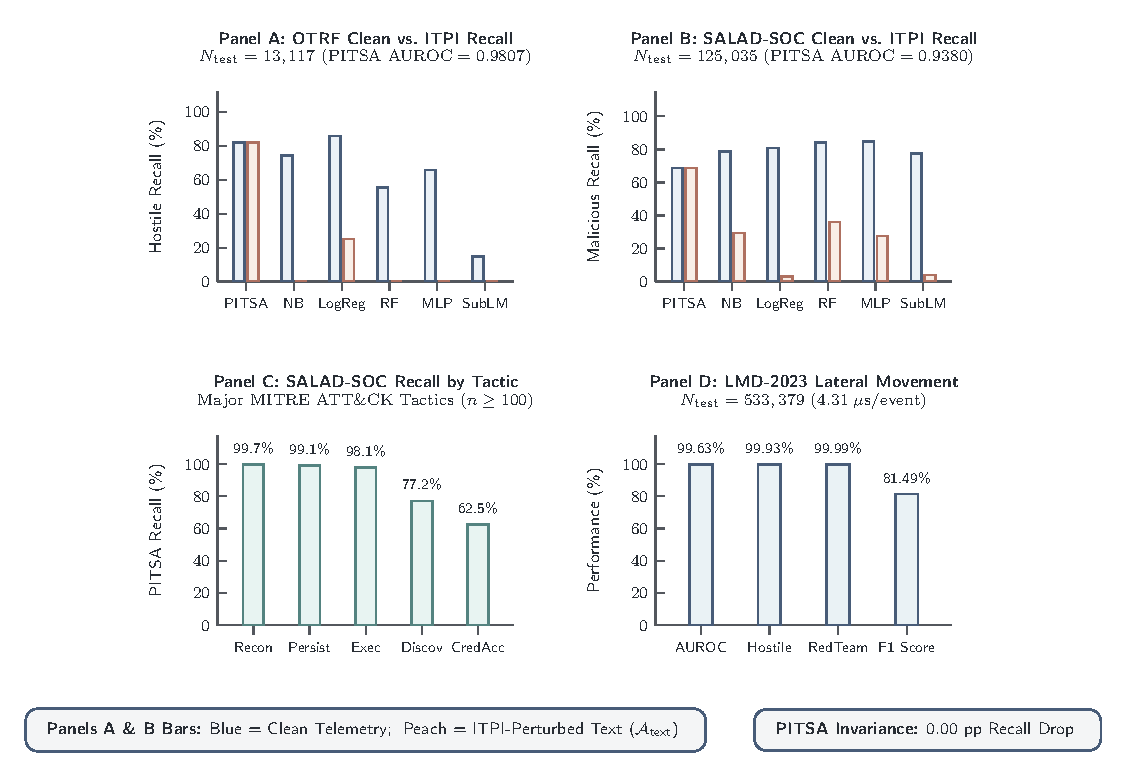
\includegraphics[width=0.92\textwidth]{figures/fig2_study1_factorial_results.pdf}
\caption{Multi-Corpus Held-Out Empirical Evaluation Across OTRF Security-Datasets ($N_{\text{test}} = 13,117$), SALAD-SOC ($N_{\text{test}} = 125,035$), and LMD-2023 ($N_{\text{test}} = 533,379$). Panels A and B compare hostile/malicious recall under Clean Telemetry (blue) versus Adversarial ITPI Text Perturbation (peach) across Partitioned PITSA and five unpartitioned baselines (Naive Bayes, Logistic Regression, Random Forest, Dense Neural MLP, and Subword LM). Panel C displays PITSA recall across major MITRE ATT\&CK tactics ($n \ge 100$) in SALAD-SOC. Panel D displays held-out LMD-2023 lateral movement detection metrics ($4.31\text{ }\mu\text{s/event}$).}
\label{fig:multicorpus_results}
\end{figure}

Panel B of \cref{tab:exp1_otrf} and Panel A of \cref{fig:pitsa_ablation} show that dropping process lineage (\texttt{AB1}) reduces OTRF recall from $81.94\%$ to $45.81\%$ ($\text{AUROC} = 0.9422$), and dropping target access masks (\texttt{AB2}) reduces recall to $69.03\%$ ($\text{AUROC} = 0.9378$), whereas relying on lineage alone (\texttt{AB6}) yields $40.65\%$ recall ($\text{AUROC} = 0.8606$), confirming that multi-pillar integration is necessary for broad coverage. Panel B of \cref{fig:pitsa_ablation} evaluates adaptive Living-off-the-Land (LOLBin) structural masking on OTRF, where an adversary progressively masks $k \in \{0, 1, 2, 3, 4, 5\}$ of the 5 structural pillars ($\rho_{\text{mask}} = k/5$) to benign modal values. Mean hostile LLR declines monotonically from $8.5651$ ($81.94\%$ recall at $k=0$, $\rho_{\text{mask}} = 0.0$) to $6.5247$ ($70.97\%$ recall at $k=1$, $\rho_{\text{mask}} = 0.2$), $3.9463$ ($49.03\%$ recall at $k=2$, $\rho_{\text{mask}} = 0.4$), $2.1620$ ($32.26\%$ recall at $k=3$, $\rho_{\text{mask}} = 0.6$), $0.2392$ ($18.06\%$ recall at $k=4$, $\rho_{\text{mask}} = 0.8$), and $-1.9922$ ($0.00\%$ recall at $k=5$, $\rho_{\text{mask}} = 1.0$), establishing the exact empirical boundary at which total 5-pillar mimicry defeats single-event structural scoring.

\begin{figure}[!htbp]
\centering
\singlespacing
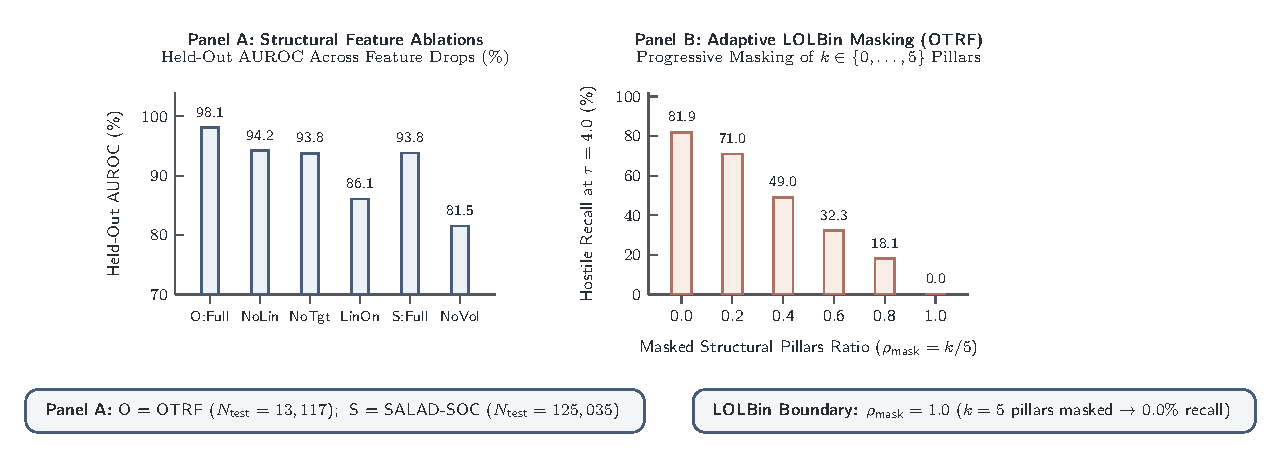
\includegraphics[width=0.92\textwidth]{figures/fig4_pitsa_ablation_and_adaptive_masking.pdf}
\caption{Structural Feature-Group Ablations and Adaptive LOLBin Structural Masking. Panel A displays held-out AUROC (\%) across feature-group drop ablations on OTRF ($N_{\text{test}} = 13,117$) and SALAD-SOC ($N_{\text{test}} = 125,035$). Panel B plots held-out OTRF hostile recall at $\tau_{\text{LLR}} = 4.0$ as an adaptive adversary progressively masks $k \in \{0, \dots, 5\}$ structural pillars ($\rho_{\text{mask}} = k/5$) to benign baseline modes.}
\label{fig:pitsa_ablation}
\end{figure}

\subsection{Experiment 2 Results: Enterprise SIEM Triage and Tactic Disaggregation on SALAD-SOC}
\label{subsec:res_exp2}

\Cref{tab:exp2_salad} and Panels B and C of \cref{fig:multicorpus_results} present the held-out evaluation on the SALAD-SOC enterprise SIEM benchmark ($N_{\text{test}} = 125,035$ alerts: $26,571$ malicious, $98,464$ benign). Executing in $384.37\text{ ms}$ total ($0.00307\text{ ms/alert}$), zero-leakage Partitioned PITSA achieves an overall $\text{AUROC} = 0.9380$ ($95\%\text{ CI}: [0.9324, 0.9401]$), $\text{Precision} = 72.50\%$, $\text{Recall} = 68.68\%$ ($18,250 / 26,571$; $95\%\text{ CI}: [68.15\%, 69.24\%]$), $\text{F1} = 0.7054$ ($95\%\text{ CI}: [0.7015, 0.7097]$), and $\text{FPR} = 7.03\%$ at $\tau_{\text{LLR}} = 1.00$ (hostile mean $\text{LLR} = 2.1827, \text{SD} = 2.3644$ vs.\ benign mean $\text{LLR} = -3.0013, \text{SD} = 2.3588$).

\begin{table}[!htbp]
\centering
\singlespacing
\caption{Experiment 2 Held-Out Results on SALAD-SOC ($N_{\text{test}} = 125,035$ Alerts): Clean, Graded Appended ITPI ($m=1$ and $m=2$), and Full ITPI Baselines, MITRE ATT\&CK Tactics, and Ablations}
\label{tab:exp2_salad}
\footnotesize
\renewcommand{\arraystretch}{0.92}
\setlength{\tabcolsep}{1.8pt}
\begin{tabular}{L{2.85cm} r c c c c c L{3.35cm}}
\toprule
\textbf{Model / Stratum / Ablation} & \textbf{Test $n$} & \textbf{Clean Rec.} & \textbf{App.\ $m=1$} & \textbf{App.\ $m=2$} & \textbf{Full ITPI} & \textbf{C-AUC / LLR} & \textbf{ITPI AUC / Significance} \\
\midrule
\multicolumn{8}{l}{\textit{Panel A: Partitioned PITSA vs.\ Five Zero-Leakage Unpartitioned Baselines ($N_{\text{test}} = 125,035$)}} \\
\textbf{PITSA Partitioned ($\tau=1.0$)} & 125,035 & \textbf{68.68\%} & \textbf{68.68\%} & \textbf{68.68\%} & \textbf{68.68\%} & \textbf{0.9380} & \textbf{0.9380 (100\% Invariant)} \\
Naive Bayes Unpartitioned & 125,035 & 78.65\% & 44.85\% & 35.80\% & 29.39\% & 0.9395 & $0.8453$ ($\chi^2=10{,}402, p<10^{-4}$) \\
Logistic Reg.\ Unpartitioned & 125,035 & 80.87\% & 20.36\% & 12.04\% & 2.92\% & 0.9653 & $0.6643$ ($\chi^2=17{,}472, p<10^{-4}$) \\
Random Forest Unpartitioned & 125,035 & 84.37\% & 35.59\% & 18.49\% & 36.05\% & 0.9690 & $0.9278$ ($\chi^2=8{,}361, p<10^{-4}$) \\
Dense Neural MLP Unpart.\ & 125,035 & 84.93\% & 77.43\% & 60.23\% & 27.53\% & 0.9686 & $0.8784$ ($\chi^2=10{,}616, p<10^{-4}$) \\
Subword LM Scorer Unpart.\ & 125,035 & 77.46\% & 10.72\% & 3.55\% & 4.03\% & 0.9581 & $0.7869$ ($\chi^2=17{,}176, p<10^{-4}$) \\
\midrule
\multicolumn{8}{l}{\textit{Panel B: PITSA Disaggregated Recall by MITRE ATT\&CK Tactic and Difficulty Level ($\tau=1.0$)}} \\
Tactic: Reconnaissance & 590 & 99.66\% & 99.66\% & 99.66\% & 99.66\% & $+4.8682$ & High-burst scan anomalies. \\
Tactic: Persistence & 109 & 99.08\% & 99.08\% & 99.08\% & 99.08\% & $+5.9980$ & Repeated-target flows captured. \\
Tactic: Execution & 1,986 & 98.14\% & 98.14\% & 98.14\% & 98.14\% & $+4.1431$ & Strong flow signature ($\text{LLR}=4.14$). \\
Tactic: Discovery & 5,420 & 77.20\% & 77.20\% & 77.20\% & 77.20\% & $+2.0323$ & Moderate-high flow separability. \\
Tactic: Command \& Control & 92 & 65.22\% & 65.22\% & 65.22\% & 65.22\% & $+0.7344$ & Partial overlap with web flows. \\
Tactic: Credential Access & 392 & 62.50\% & 62.50\% & 62.50\% & 62.50\% & $+1.0019$ & Burst authentication flows. \\
Tactic: Impact & 15,197 & 55.41\% & 55.41\% & 55.41\% & 55.41\% & $+1.1686$ & Volumetric traffic overlap. \\
Tactic: Init.\ Access \& Lat.\ Mov.\ & 97 & 9.28\% & 9.28\% & 9.28\% & 9.28\% & $+0.2971$ & Low-volume web/internal flows. \\
Difficulty: Hard Malicious & 8,698 & 85.74\% & 85.74\% & 85.74\% & 85.74\% & $+3.5487$ & Highest structural LLR separation. \\
Difficulty: Medium Malicious & 17,725 & 60.83\% & 60.83\% & 60.83\% & 60.83\% & $+1.5304$ & Intermediate flow separability. \\
\midrule
\multicolumn{8}{l}{\textit{Panel C: SALAD-SOC Feature-Group Ablations ($\tau=1.0$)}} \\
AB1: Drop Protocol/Port (\texttt{s1}) & 125,035 & 64.13\% & 64.13\% & 64.13\% & 64.13\% & 0.8965 & $\Delta\text{AUROC} = -0.0415$; $\text{FPR}=10.44\%$. \\
AB2: Drop Flow Volume (\texttt{s2}) & 125,035 & 36.91\% & 36.91\% & 36.91\% & 36.91\% & 0.8151 & Largest drop ($\Delta\text{AUROC} = -0.1229$). \\
\bottomrule
\end{tabular}
\end{table}

On SALAD-SOC (\cref{tab:exp2_salad}, Panel A), under Clean Telemetry ($m=0$), combining pre-triage SIEM session log text with structural flow pillars allows the unpartitioned baselines to achieve strong initial recall ($84.93\%$ for Dense Neural MLP, $84.37\%$ for Random Forest, $80.87\%$ for Logistic Regression, $78.65\%$ for Naive Bayes, and $77.46\%$ for Subword LM, with clean AUROC values from $0.9395$ to $0.9690$). However, this reliance on $\mathcal{A}_{\text{text}}$ exposes every unpartitioned architecture to severe, graded degradation under Indirect Telemetry Prompt Injection:
\begin{itemize}
  \item Under \textbf{Graded Appended ITPI}, where the original pre-triage rule candidate is $100\%$ preserved and $m \in \{1, 2, 4, 8\}$ benign session clauses are appended, Logistic Regression recall drops from $80.87\%$ ($m=0$) to $20.36\%$ ($m=1$), $12.04\%$ ($m=2$), $2.99\%$ ($m=4$), and $0.77\%$ ($m=8$); Subword LM drops from $77.46\%$ to $10.72\%$ ($m=1$), $3.55\%$ ($m=2$), $3.15\%$ ($m=4$), and $3.00\%$ ($m=8$); Naive Bayes drops from $78.65\%$ to $44.85\%$ ($m=1$), $35.80\%$ ($m=2$), $32.97\%$ ($m=4$), and $25.65\%$ ($m=8$); Random Forest drops from $84.37\%$ to $35.59\%$ ($m=1$) and $18.49\%$ ($m=2$); and Dense Neural MLP degrades progressively from $84.93\%$ to $77.43\%$ ($m=1$), $60.23\%$ ($m=2$), $29.96\%$ ($m=4$), and $25.14\%$ ($m=8$).
  \item Under \textbf{Full ITPI}, recall falls to $2.92\%$ for Logistic Regression ($\text{ITPI AUROC} = 0.6643$), $4.03\%$ for Subword LM ($\text{ITPI AUROC} = 0.7869$), $27.53\%$ for Dense Neural MLP ($\text{ITPI AUROC} = 0.8784$), $29.39\%$ for Naive Bayes ($\text{ITPI AUROC} = 0.8453$), and $36.05\%$ for Random Forest ($\text{ITPI AUROC} = 0.9278$). Paired McNemar's discordant-pair tests confirm that PITSA's held-out recall under ITPI ($68.68\%$) achieves a statistically significant recall advantage over all five unpartitioned baselines ($\chi^2 = 8,361.46$ to $17,472.00$, all $p < 0.0001$).
\end{itemize}
Across all ITPI regimes, Partitioned PITSA maintains $68.68\%$ overall recall and $85.74\%$ recall on \texttt{hard} malicious alerts, including $99.66\%$ on Reconnaissance, $99.08\%$ on Persistence, $98.14\%$ on Execution, and $77.20\%$ on Discovery tactics (\cref{tab:exp2_salad}, Panel B), while combined low-volume \texttt{Initial Access \& Lateral Movement} alerts ($n=97$) exhibit $9.28\%$ single-flow recall ($\text{mean LLR} = +0.2971$; $2.22\%$ on Initial Access $n=90$ and $100.00\%$ on Lateral Movement $n=7$). Dropping packet/byte flow volume (\texttt{AB2}) causes the largest single-pillar degradation ($\Delta \text{AUROC} = -0.1229$, recall $68.68\% \to 36.91\%$; \cref{tab:exp2_salad}, Panel C).

\subsection{Experiment 3 Results: Large-Scale Lateral Movement Detection on LMD-2023 and CISA KEV}
\label{subsec:res_exp3}

\Cref{tab:exp3_lmd} and Panel D of \cref{fig:multicorpus_results} report the held-out evaluation on the $1,777,930$-row LMD-2023 Windows Sysmon benchmark ($N_{\text{test}} = 533,379$ events: $483,491$ Normal, $33,224$ standard Malicious, and $16,664$ RedTeam lateral movement events). Scoring all $533,379$ held-out events in $2,299.93\text{ ms}$ ($4.3120\text{ }\mu\text{s/event}$, or $231,910$ events per second), Partitioned PITSA achieves an overall $\text{AUROC} = 0.9963$ ($95\%\text{ CI}: [0.9961, 0.9969]$; hostile mean $\text{LLR} = 15.8780, \text{SD} = 5.1904$; RedTeam mean $\text{LLR} = 10.7773, \text{SD} = 5.0992$; Normal mean $\text{LLR} = -21.2220, \text{SD} = 8.5267$).

\begin{table}[!htbp]
\centering
\singlespacing
\caption{Experiment 3 Held-Out Results on LMD-2023 Lateral Movement Sysmon Corpus ($N_{\text{test}} = 533,379$ Events): Threshold Sweep and Structural Feature-Group Ablations}
\label{tab:exp3_lmd}
\footnotesize
\setlength{\tabcolsep}{2.5pt}
\begin{tabular}{L{3.5cm} c c c c c c L{3.1cm}}
\toprule
\textbf{Configuration / Ablation} & \textbf{Prec.} & \textbf{Host.\ Rec.} & \textbf{RT Rec.} & \textbf{F1} & \textbf{FPR} & \textbf{AUROC} & \textbf{Confusion Matrix / Role} \\
\midrule
\multicolumn{8}{l}{\textit{Panel A: Operating Threshold Sweep on Held-Out LMD-2023 ($N_{\text{test}} = 533,379$)}} \\
$\tau_{\text{LLR}} = 0.0$ & 0.6878 & 0.9993 & 0.9999 & 0.8148 & 0.0468 & 0.9963 & $\text{TP}=49{,}854,\; \text{FN}=34$ \\
\textbf{$\tau_{\text{LLR}} = 0.5$ (Primary Gate)} & \textbf{0.6879} & \textbf{0.9993} & \textbf{0.9999} & \textbf{0.8149} & \textbf{0.0468} & \textbf{0.9963} & \textbf{Captures $99.99\%$ RedTeam.} \\
$\tau_{\text{LLR}} = 1.0$ & 0.6884 & 0.9991 & 0.9992 & 0.8152 & 0.0467 & 0.9963 & $\text{TP}=49{,}843,\; \text{FN}=45$ \\
$\tau_{\text{LLR}} = 2.0$ & 0.6927 & 0.9969 & 0.9930 & 0.8174 & 0.0456 & 0.9963 & $\text{TP}=49{,}735,\; \text{FN}=153$ \\
$\tau_{\text{LLR}} = 4.0$ & 0.7026 & 0.9839 & 0.9550 & 0.8198 & 0.0430 & 0.9963 & $\text{TP}=49{,}087,\; \text{FN}=801$ \\
\midrule
\multicolumn{8}{l}{\textit{Panel B: Structural Feature-Group Ablations at $\tau_{\text{LLR}} = 0.50$}} \\
AB1: Drop Process Lineage (\texttt{p1}) & 0.6834 & 0.9986 & 0.9969 & 0.8115 & 0.0477 & 0.9958 & $\text{FN}$ doubles ($34 \to 72$). \\
AB2: Drop Reg./File EID (\texttt{p2}) & 0.6879 & 0.9993 & 0.9999 & 0.8149 & 0.0468 & 0.9963 & Redundant with \texttt{p1}/\texttt{p3} on LMD. \\
AB3: Drop Net/Pipe EID (\texttt{p3}) & 0.6912 & 0.9982 & 0.9969 & 0.8168 & 0.0460 & 0.9973 & $\text{FN}$ rises from $34$ to $91$. \\
AB4: Drop Dest Port (\texttt{p4}) & 0.6926 & 0.9947 & 0.9863 & 0.8166 & 0.0456 & 0.9962 & $\text{FN}$ rises $7.8\times$ ($34 \to 264$). \\
AB5: Drop Host/Station (\texttt{p5}) & 0.6089 & 0.9971 & 0.9991 & 0.7561 & 0.0661 & 0.9952 & $\text{FP}$ rises by $+9{,}332$ ($+41.3\%$). \\
\bottomrule
\end{tabular}
\end{table}

At the primary gate $\tau_{\text{LLR}} = 0.50$, PITSA detects $49,854$ of $49,888$ held-out hostile events ($99.93\%$ overall hostile recall, $95\%\text{ CI}: [99.91\%, 99.95\%]$, missing only $34$ events across half a million records) and captures $99.99\%$ of RedTeam lateral movement events ($99.90\%$ of standard malicious events) at a false positive rate of $4.68\%$ ($\text{Precision} = 68.79\%, \text{F1} = 0.8149, 95\%\text{ CI}: [0.8131, 0.8168]$). Ablating destination port service profiles (\texttt{AB4\_NoDestPort}) increases false negatives by $7.8\times$ (from $34$ to $264$ and reduces RedTeam recall from $99.99\%$ to $98.63\%$), while ablating computer station topology (\texttt{AB5\_NoHostUserContext}) increases false positives from $22,618$ to $31,950$ ($\text{FPR} = 6.61\%, \text{F1} = 0.7561$). Complementary analysis of the $1,741$ actively exploited CVEs in the CISA KEV catalog confirms that $361$ vulnerabilities ($20.74\%$) are actively used in known ransomware campaigns, concentrated heavily in enterprise infrastructure vendors (Microsoft: $390$ CVEs, Cisco: $100$, Apple: $95$, Adobe: $82$, Google: $75$), reinforcing why lateral-movement and privilege-escalation telemetry cannot be safely delegated to unverified LLM prose \citep{li2022assessing, ampel2024improving}.

\subsection{Experiment 4 Results: Trace-Driven Decision-Theoretic Sensitivity, Dominance Boundaries \texorpdfstring{($\kappa^*$)}{(kappa*)}, and Endogenous Habituation}
\label{subsec:res_exp4}

To answer \textbf{RQ2} and \textbf{RQ3} without fabricating human-subject trials, we evaluated the four formal governance policies ($\Pi_1$ Disfluent Baseline, $\Pi_2$ Unassisted Fluent LLM Triage, $\Pi_3$ Static Warning Banner on All Alerts, and $\Pi_4$ Selective Two-Stage DECS Gated by PITSA) directly over the held-out empirical PITSA log-likelihood distributions from OTRF ($13,117$ events, $\tau_{\text{LLR}} = 4.0$) and SALAD-SOC ($125,035$ alerts, $\tau_{\text{LLR}} = 1.0$). \Cref{tab:exp4_dcedm} and \cref{fig:dcedm_sensitivity} present the trace-driven sensitivity results across $\lambda_F \in [0.0, 0.6]$, cost ratios $c_{\text{miss}} / c_V \in \{5, 10, 20, 50, 100\}$, and the unified endogenous habituation law $\gamma_{\text{eff}}(\tau_{\text{LLR}}) = 1.80 \exp(-2.10 \cdot \text{BFR}(\tau_{\text{LLR}}))$.

\begin{table}[!htbp]
\centering
\singlespacing
\caption{Experiment 4 Trace-Driven Analytical Decision-Theoretic Evaluation Across Held-Out OTRF ($N_{\text{test}}=13,117$) and SALAD-SOC ($N_{\text{test}}=125,035$): CMR, Expected Loss, and Unified Endogenous Habituation Sweep}
\label{tab:exp4_dcedm}
\footnotesize
\setlength{\tabcolsep}{2.2pt}
\begin{tabular}{L{2.9cm} c c c c c c}
\toprule
\textbf{Trace / Parameter} & \textbf{$\Pi_1$ Disfl.} & \textbf{$\Pi_2$ Fluent} & \textbf{$\Pi_3$ Static} & \textbf{$\Pi_4$ DECS} & \textbf{Trap ($\Pi_2-\Pi_1$)} & \textbf{Gain ($\Pi_2-\Pi_4$)} \\
\midrule
\multicolumn{7}{l}{\textit{Panel A: Held-Out OTRF Compromise Miss Rate (CMR) vs.\ $\lambda_F$ ($\tau_{\text{LLR}}=4.0$, Banner Rate $= 4.08\%$)}} \\
$\lambda_F = 0.0$ (Zero Fluency) & 13.91\% & 13.91\% & 13.91\% & 8.73\% & $+0.00\text{ pp}$ & $-5.17\text{ pp}$ \\
$\lambda_F = 0.2$ (Low Bias) & 13.91\% & 20.40\% & 18.80\% & 9.57\% & $+6.49\text{ pp}$ & $-10.83\text{ pp}$ \\
\textbf{$\lambda_F = 0.4$ (Canonical)} & \textbf{13.91\%} & \textbf{28.88\%} & \textbf{24.90\%} & \textbf{10.43\%} & \textbf{$+14.97\text{ pp}$} & \textbf{$-18.45\text{ pp}$} \\
$\lambda_F = 0.6$ (High Bias) & 13.91\% & 39.23\% & 32.21\% & 11.31\% & $+25.33\text{ pp}$ & $-27.93\text{ pp}$ \\
\midrule
\multicolumn{7}{l}{\textit{Panel B: Held-Out SALAD-SOC Compromise Miss Rate (CMR) vs.\ $\lambda_F$ ($\tau_{\text{LLR}}=1.0$, Banner Rate $= 20.13\%$)}} \\
$\lambda_F = 0.0$ (Zero Fluency) & 36.00\% & 36.00\% & 36.00\% & 21.10\% & $+0.00\text{ pp}$ & $-14.90\text{ pp}$ \\
$\lambda_F = 0.2$ (Low Bias) & 36.00\% & 49.02\% & 46.10\% & 22.91\% & $+13.02\text{ pp}$ & $-26.11\text{ pp}$ \\
\textbf{$\lambda_F = 0.4$ (Canonical)} & \textbf{36.00\%} & \textbf{62.02\%} & \textbf{56.41\%} & \textbf{24.70\%} & \textbf{$+26.02\text{ pp}$} & \textbf{$-37.32\text{ pp}$} \\
$\lambda_F = 0.6$ (High Bias) & 36.00\% & 73.46\% & 66.15\% & 26.44\% & $+37.46\text{ pp}$ & $-47.03\text{ pp}$ \\
\midrule
\multicolumn{7}{l}{\textit{Panel C: Held-Out SALAD-SOC Expected Loss $\mathcal{L}(\Pi)$ Across $c_{\text{miss}}/c_V$ ($\lambda_F = 0.40$, Crossover $\kappa^* = 1.68$)}} \\
$c_{\text{miss}} / c_V = 5$ & 0.7997 & 0.9099 & 0.8855 & 0.6355 & $+13.78\%$ & $-30.16\%$ \\
$c_{\text{miss}} / c_V = 10$ & 1.2384 & 1.6104 & 1.5302 & 0.9364 & $+30.04\%$ & $-41.85\%$ \\
\textbf{$c_{\text{miss}} / c_V = 20$ (Canonical)} & \textbf{1.9075} & \textbf{2.8201} & \textbf{2.6171} & \textbf{1.4125} & \textbf{$+47.84\%$} & \textbf{$-49.91\%$} \\
$c_{\text{miss}} / c_V = 50$ & 3.3295 & 5.7700 & 5.1916 & 2.4782 & $+73.30\%$ & $-57.05\%$ \\
$c_{\text{miss}} / c_V = 100$ & 5.0092 & 9.6860 & 8.5188 & 3.7995 & $+93.36\%$ & $-60.77\%$ \\
\midrule
\multicolumn{7}{l}{\textit{Panel D: Unified Endogenous Habituation Sweep $\gamma_{\text{eff}}(\tau)$ on OTRF ($c_{\text{miss}}/c_V=50, \lambda_F=0.40, \kappa^*=39.64$)}} \\
\textbf{Threshold $\tau_{\text{LLR}}$} & \textbf{BFR($\tau$)} & \textbf{$\gamma_{\text{eff}}(\tau)$} & \textbf{CMR($\tau$)} & \textbf{Loss $\mathcal{L}(\tau)$} & \textbf{vs.\ $\Pi_3$} & \textbf{Regime} \\
$\tau \to -\infty$ (Static $\Pi_3$) & 100.00\% & 0.2204 & 19.27\% & 0.2431 & $+0.00\%$ & Habituation decay \\
$\tau_{\text{LLR}} = 0.0$ & 9.57\% & 1.4724 & 6.04\% & 0.2286 & $-5.96\%$ & High sensitivity \\
\textbf{$\tau^*_{\text{LLR}} = 1.0$ (Optimum)} & \textbf{6.49\%} & \textbf{1.5707} & \textbf{5.70\%} & \textbf{0.2199} & \textbf{$-9.54\%$} & \textbf{Interior optimum} \\
$\tau_{\text{LLR}} = 2.0$ & 5.59\% & 1.6007 & 7.12\% & 0.2265 & $-6.83\%$ & Near-optimal \\
$\tau_{\text{LLR}} = 4.0$ & 4.08\% & 1.6522 & 8.66\% & 0.2334 & $-3.99\%$ & Low banner ($4.1\%$) \\
$\tau_{\text{LLR}} = 6.0$ & 1.06\% & 1.7604 & 10.59\% & 0.2429 & $-0.08\%$ & Marginal gain \\
$\tau_{\text{LLR}} = 8.0$ (Over-Tight) & 0.72\% & 1.7731 & 11.16\% & 0.2462 & $+1.28\%$ & Backfire ($>\Pi_3$) \\
\bottomrule
\end{tabular}
\end{table}

Four core decision-theoretic insights emerge from \cref{tab:exp4_dcedm} and \cref{fig:dcedm_sensitivity}, directly validating \cref{thm:dcedm_dominance} and \cref{cor:dominance_boundary}:
\begin{enumerate}
  \item \textbf{Drastic Reduction in Warning Banner Overhead:} Whereas Policy $\Pi_3$ (Static Warning Banner) displays a caution banner on $100.00\%$ of events, Policy $\Pi_4$ (Selective DECS gated by PITSA) triggers a rebuttal banner on only $4.08\%$ of OTRF events at $\tau_{\text{LLR}} = 4.0$ ($95.92\%$ reduction in banner volume) and $20.13\%$ of SALAD-SOC alerts at $\tau_{\text{LLR}} = 1.0$ ($79.87\%$ reduction in banner volume).
  \item \textbf{Mitigation of the Epistemic Fluency Trap Across $\lambda_F$:} On the OTRF stream (Panel A), increasing fluency susceptibility from $\lambda_F = 0.0$ to $\lambda_F = 0.40$ inflates the Compromise Miss Rate under unassisted fluent triage ($\Pi_2$) by $+14.97\text{ pp}$ (from $13.91\%$ to $28.88\%$), and up to $39.23\%$ ($+25.33\text{ pp}$) at $\lambda_F = 0.60$. Because static banners ($\Pi_3$) suffer habituation decay ($\gamma_{\text{hab}} = 0.22$), $\text{CMR}(\Pi_3)$ still reaches $24.90\%$ at $\lambda_F = 0.40$. In contrast, Selective DECS ($\Pi_4$) holds $\text{CMR}$ to $10.43\%$ at $\lambda_F = 0.40$ ($-18.45\text{ pp}$ reduction relative to $\Pi_2$). On SALAD-SOC (Panel B and \cref{fig:dcedm_sensitivity}A), fluency susceptibility at $\lambda_F = 0.40$ inflates $\text{CMR}(\Pi_2)$ from $36.00\%$ to $62.02\%$ ($+26.02\text{ pp}$), whereas Selective DECS ($\Pi_4$) reduces $\text{CMR}$ to $24.70\%$ ($-37.32\text{ pp}$ risk reduction).
  \item \textbf{Exact Cost-Ratio Crossover Boundaries $\kappa^*(\lambda_F)$ (\Cref{cor:dominance_boundary}(2) and \cref{fig:dcedm_sensitivity}C):} Confirming that DECS dominance is not tautologically built into the equations, on the low-base-rate OTRF host stream ($p_1 = 1.18\%$), the critical crossover cost ratio is $\kappa^*(0.10) = 33.54$, $\kappa^*(0.20) = 48.90$, $\kappa^*(0.30) = 47.35$, $\kappa^*(0.40) = 39.64$, $\kappa^*(0.50) = 31.56$, and $\kappa^*(0.60) = 24.88$. Thus, at $\lambda_F = 0.40$, whenever the organizational cost ratio satisfies $c_{\text{miss}}/c_V < 39.64$, Selective DECS ($\Pi_4$) incurs \emph{higher} expected operational loss than Unassisted Fluent Triage ($\Pi_2$) ($0.1066$ vs.\ $0.0745$ at $c_{\text{miss}}/c_V = 5$; $0.1332$ vs.\ $0.1057$ at $c_{\text{miss}}/c_V = 10$; $0.1685$ vs.\ $0.1507$ at $c_{\text{miss}}/c_V = 20$), and strictly dominates only in high-consequence regimes where $c_{\text{miss}}/c_V > 39.64$ ($0.2340$ vs.\ $0.2427$ at $c_{\text{miss}}/c_V = 50$, a $-3.60\%$ loss reduction; and $0.3036$ vs.\ $0.3500$ at $c_{\text{miss}}/c_V = 100$, a $-13.25\%$ loss reduction). On SALAD-SOC ($p_1 = 21.25\%$, Panel C and \cref{fig:dcedm_sensitivity}B and C), the critical crossover is $\kappa^*(0.40) = 1.68$, so $\Pi_4$ reduces expected loss across all $c_{\text{miss}}/c_V \in [5, 100]$ by $30.16\%$ to $60.77\%$.
  \item \textbf{Interior U-Shaped Optimal Threshold Under Unified Endogenous Habituation (\Cref{cor:dominance_boundary}(3) and \cref{fig:dcedm_sensitivity}D):} Panel D of \cref{tab:exp4_dcedm} and \cref{fig:dcedm_sensitivity}D evaluate both $\Pi_3$ and $\Pi_4(\tau_{\text{LLR}})$ under the single endogenous habituation law $\gamma_{\text{eff}}(\tau_{\text{LLR}}) = 1.80 \exp(-2.10 \cdot \text{BFR}(\tau_{\text{LLR}}))$ on OTRF ($c_{\text{miss}}/c_V = 50, \lambda_F = 0.40$). At $\tau_{\text{LLR}} \to -\infty$ (Static Banner $\Pi_3$), $\text{BFR} = 100.00\%$ drives $\gamma_{\text{eff}}$ down to $0.2204$, yielding $\text{CMR} = 19.27\%$ and $\mathcal{L} = 0.2431$. Raising $\tau_{\text{LLR}}$ to the interior optimum $\tau^*_{\text{LLR}} = 1.0$ cuts $\text{BFR}$ to $6.49\%$, restoring $\gamma_{\text{eff}} = 1.5707$, reducing $\text{CMR}$ to $5.70\%$, and achieving the global minimum expected loss $\mathcal{L}(1.0) = 0.2199$ ($-9.54\%$ below $\Pi_3$). However, raising $\tau_{\text{LLR}}$ too far to $\tau_{\text{LLR}} = 8.0$ ($\text{BFR} = 0.72\%, \gamma_{\text{eff}} = 1.7731$) leaves $39.35\%$ of hostile events uncontested, causing $\text{CMR}$ to rebound to $11.16\%$ and driving expected loss up to $\mathcal{L}(8.0) = 0.2462 > \mathcal{L}(\Pi_3) = 0.2431$ ($+1.28\%$ backfire).
\end{enumerate}

\begin{figure}[!htbp]
\centering
\singlespacing
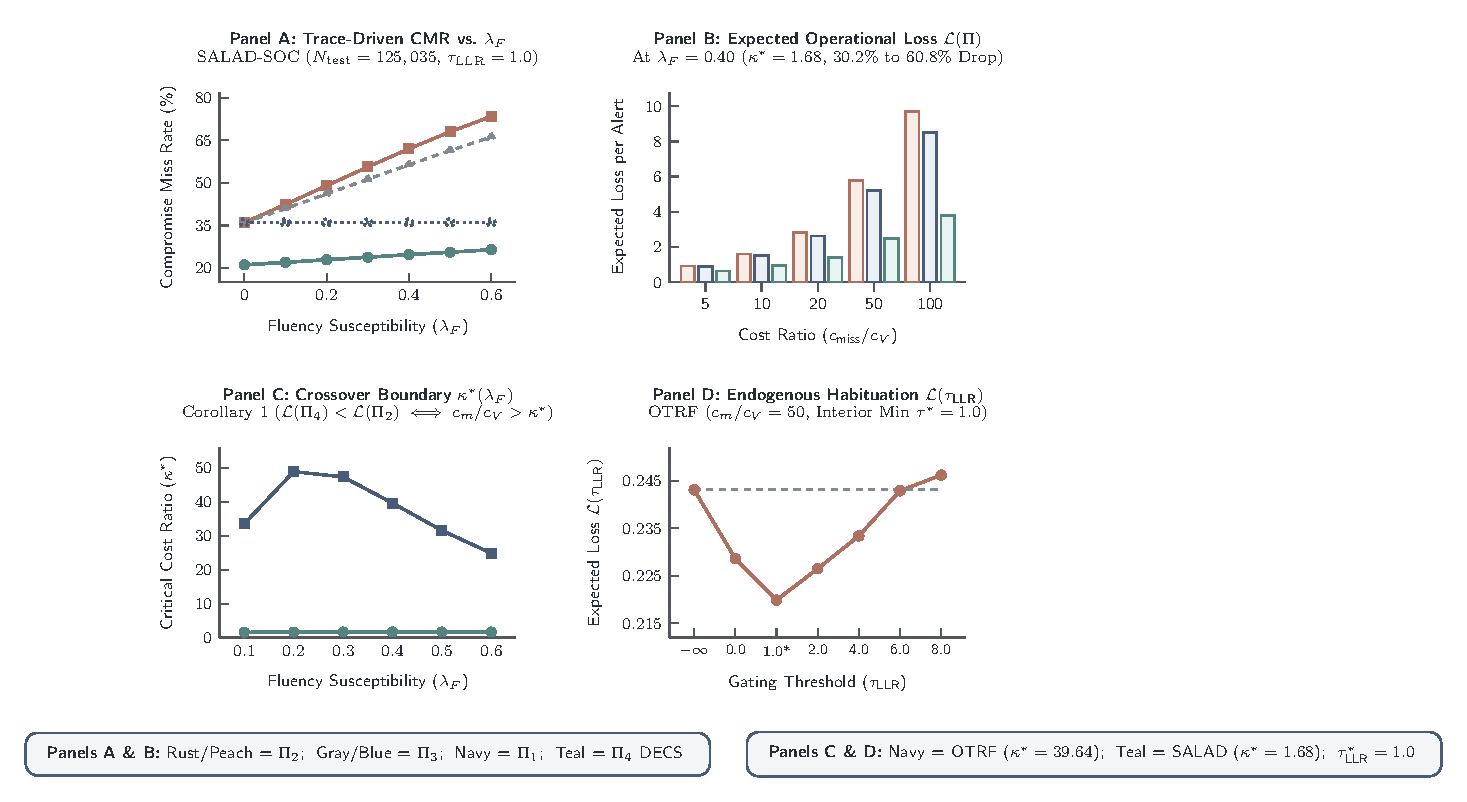
\includegraphics[width=0.92\textwidth]{figures/fig3_study1b_mechanism_and_habituation.pdf}
\caption{Experiment 4 Trace-Driven Analytical Decision-Theoretic Evaluation Across Held-Out SALAD-SOC ($N_{\text{test}} = 125,035$) and OTRF ($N_{\text{test}} = 13,117$). Panel A plots expected Compromise Miss Rate (CMR, \%) across fluency susceptibility $\lambda_F \in [0.0, 0.6]$ on SALAD-SOC ($\tau_{\text{LLR}} = 1.0$). Panel B compares Expected Operational Loss per Alert $\mathcal{L}(\Pi)$ at $\lambda_F = 0.40$ across asymmetric cost ratios $c_{\text{miss}}/c_V \in \{5, 10, 20, 50, 100\}$. Panel C plots the Corollary 1 critical cost-ratio crossover boundary $\kappa^*(\lambda_F)$ on OTRF ($\kappa^*(0.40)=39.64$) and SALAD-SOC ($\kappa^*(0.40)=1.68$). Panel D plots the unified endogenous habituation curve $\mathcal{L}(\tau_{\text{LLR}})$ on OTRF ($c_{\text{miss}}/c_V = 50$), demonstrating the interior U-shaped minimum at $\tau^*_{\text{LLR}} = 1.0$.}
\label{fig:dcedm_sensitivity}
\end{figure}

\section{Discussion and Conclusion}
\label{sec:discussion}

\subsection{Synthesis of Findings and Theoretical Implications for Information Systems}
\label{subsec:disc_theory}

This study investigated how untrusted telemetry text channels and generative rationale fluency interact to create an epistemic fluency trap in AI-augmented security operations, and how architectural text/telemetry partitioning paired with selective defeasible cueing restores detection invariance and decision-theoretic resilience. Across $2,238,434$ real telemetry records ($671,531$ held-out test records), we established that five unpartitioned classifiers spanning lexical, dense semantic neural MLP, and contextual subword language model architectures suffer severe, statistically significant recall collapse under both graded appended and full-override Indirect Telemetry Prompt Injection ($85.81\% \to 30.32\% \to 25.16\%$ for Logistic Regression and $65.81\% \to 8.39\% \to 0.00\%$ for Dense Neural MLP on OTRF; $77.46\%\text{ to }84.93\%$ clean recall dropping to $2.92\%\text{ to }36.05\%$ under ITPI on SALAD-SOC; McNemar's $\chi^2 \ge 86.01$ on OTRF and $\chi^2 \ge 8,361.46$ on SALAD-SOC, all $p < 0.0001$), whereas Partitioned PITSA maintains $0.00\text{ pp}$ degradation ($\text{AUROC} = 0.9807$ on OTRF, $0.9380$ on SALAD-SOC, and $0.9963$ on LMD-2023 at $2.12$ to $4.31\text{ }\mu\text{s}$ per event). These findings advance Information Systems scholarship in \textit{Journal of Management Information Systems} and the broader decision-support literature across three interconnected fronts \citep{chatterjee2020need, diaz2023indigenous, tutun2024explainable, ansari2026partner}.

First, the \textbf{Dual-Cue Epistemic Defeasibility Model (DCEDM)} (\cref{thm:dcedm_dominance} and \cref{cor:dominance_boundary}) extends IS human-AI delegation, role configuration, and explainability theory \citep{baird2021next, fugener2022cognitive, revilla2023human, tutun2024explainable, ansari2026partner, bag2025enhancing, taudien2026effect} into adversarially contested environments. Prevailing IS delegation and narrative XAI models treat AI explanations as benign informational signals whose linguistic coherence monotonically aids comprehension and human metaknowledge \citep{burton2020systematic, bag2025enhancing, taudien2026effect}. By integrating metacognitive processing fluency theory \citep{alter2009uniting} with cost-benefit verification allocation \citep{vasconcelos2023explanations, bucinca2021trust} and analytical security economics \citep{liu2020centralized, li2021roles}, DCEDM formalizes why linguistic coherence acts as an epistemic sedative when the explanation generator itself is exposed to adversarial text inputs: high narrative fluency ($\Delta F = 0.70$) shifts posterior compromise log-odds downward and inflates expected Compromise Miss Rates by $+14.97\text{ pp}$ on OTRF and $+26.02\text{ pp}$ on SALAD-SOC at $\lambda_F = 0.40$. Moreover, \cref{cor:dominance_boundary} establishes exact boundary conditions ($\kappa^* = 39.64$ on low-base-rate OTRF vs.\ $\kappa^* = 1.68$ on SALAD-SOC) delineating when selective contestation is cost-effective versus when low miss-to-verification cost ratios render unassisted triage preferable.

Second, our proof of \cref{prop:partition_invariance}, our three socio-technical design principles (\textbf{DP1 to DP3}), and our multi-corpus empirical evaluations advance computational cybersecurity design science in \textit{JMIS} \citep{lowry2017security, ebrahimi2020semi, li2022assessing, naseer2023enabling, ampel2024improving, srinivas2025ai}. We demonstrate that the vulnerability of AI-assisted triage to Indirect Telemetry Prompt Injection is not merely a prompt-engineering quirk of large language models, nor is it resolved by replacing bag-of-words features with dense neural embeddings (\texttt{DenseNeuralMLP}) or contextual subword sequence models (\texttt{SubwordLM}). Rather, it is a fundamental structural property of any unpartitioned classifier ($\mathcal{A}_{\text{struct}} \oplus \mathcal{A}_{\text{text}}$) that allows adversary-controlled string tokens to inject negative log-odds weight against kernel and flow indicators, even when the original malicious command string or pre-triage rule candidate remains $100\%$ intact under graded appended injection ($m \ge 1$). Enforcing the projection operator $\Pi_{\text{struct}}$ (\textbf{DP1}) and white-box additive evidence decomposition (\textbf{DP2}) eliminates text-channel dilution while providing exact per-pillar forensic attribution ($k^*(e)$) at microsecond CPU latency.

Third, our unified endogenous habituation analysis (\cref{cor:dominance_boundary} and \cref{tab:exp4_dcedm}, Panel D) extends neuro-cognitive security and warning habituation research \citep{anderson2016warning, vance2018fog, cram2021technostress, jensen2022improving, hsu2024proactive, tarafdar2017technostress, bartal2026alert} by demonstrating that selective contestation threshold calibration ($\tau_{\text{LLR}}$) is a non-trivial interior optimization problem (\textbf{DP3}). Under a single exponential habituation law $\gamma_{\text{eff}}(\tau_{\text{LLR}}) = \gamma_0 \exp(-\eta_{\text{hab}} \cdot \text{BFR}(\tau_{\text{LLR}}))$, setting $\tau_{\text{LLR}} \to -\infty$ (static banners) fails due to severe habituation ($\text{BFR} = 100\%, \mathcal{L} = 0.2431$), whereas setting $\tau_{\text{LLR}} = 8.0$ fails due to uncontested hostile misses ($\mathcal{L} = 0.2462 > \mathcal{L}(\Pi_3)$), with the interior optimum achieved at $\tau^*_{\text{LLR}} \in [1.0, 4.0]$ ($\mathcal{L}(1.0) = 0.2199$).

\subsection{Practical, Managerial, and SOC Governance Implications}
\label{subsec:disc_practice}

For enterprise CISOs, SIEM/XDR architects, and SOC managers \citep{liu2020centralized, li2021roles, davison2025research}, our findings yield three actionable governance implications:
\begin{enumerate}
  \item \textbf{SIEM/XDR Engineering Implication (Mandatory Text and Telemetry Air-Gapping, DP1 \& DP2):} Because concatenating untrusted text fields with structural telemetry causes $48.32\text{ pp}$ to $77.95\text{ pp}$ recall collapse on SALAD-SOC and $55.49\text{ pp}$ to $74.19\text{ pp}$ recall collapse on OTRF under graded appended and full-override ITPI across lexical, dense neural MLP, and subword language models, security engineering teams should never rely on unpartitioned classifiers or LLM self-critique prompts as safety gates. Deploying Partitioned PITSA requires zero GPU hardware, adds only $2.12$ to $4.31\text{ }\mu\text{s}$ per event, and ensures mathematical invariance to text-channel prompt injection.
  \item \textbf{SOC Interface Governance Implication (Cost-Ratio and Interior Threshold Calibration, DP3):} SOC managers should replace persistent ``AI can make mistakes'' disclaimers with the Two-Stage DECS workflow, calibrating deployment to the stream's base rate and cost ratio (\cref{cor:dominance_boundary}). On high-priority SIEM alert streams ($p_1 \approx 21\%, \kappa^* = 1.68$), DECS dominates across all operational cost regimes at $\tau_{\text{LLR}} = 1.0$. On raw host telemetry streams ($p_1 \approx 1.2\%, \kappa^* = 39.64$), DECS should be deployed for high-consequence assets ($c_{\text{miss}}/c_V \ge 40$) with $\tau_{\text{LLR}} \in [1.0, 4.0]$ to capture the interior habituation minimum while avoiding over-conservative backfire ($\tau_{\text{LLR}} = 8.0$).
  \item \textbf{Audit and Compliance Implication (Structural Defeater Provenance, NIST CSF 2.0 RS.AN-06):} To prevent unverified closure of contested alerts, SIEM ticketing systems should automatically append PITSA's log-likelihood ratio $L(e)$ and primary structural defeater pillar $k^*(e)$ to the immutable audit log whenever an operator dismisses an alert with $L(e) > \tau_{\text{LLR}}$.
\end{enumerate}

\subsection{Limitations, Scope Boundaries, and Future Research}
\label{subsec:disc_limitations}

Two explicit scope boundaries govern our findings and define priorities for future research. First, regarding \textbf{normative analytical modeling versus human-subject trials}, while Experiments 1 through 3 evaluate real host and network telemetry across $2,238,434$ records and Experiment 4 evaluates governance policies via a trace-driven normative Bayesian decision-theoretic model parameterized by published cognitive fluency and neuro-cognitive habituation studies \citep{alter2009uniting, anderson2016warning, vance2018fog, vasconcelos2023explanations, bag2025enhancing}, this study did not conduct live human-in-the-loop experiments or practitioner interviews. Normative analytical models provide exact, reproducible sensitivity surfaces and closed-form dominance boundaries ($\kappa^*(\lambda_F)$ and $\tau^*_{\text{LLR}}$) across $\lambda_F \in [0.0, 0.6]$ and $c_{\text{miss}}/c_V \in [5, 100]$, but cannot capture interpersonal team escalation dynamics, shift-handover fatigue, or organizational politics inside live SOCs \citep{revilla2023human, bartal2026alert}. Future empirical research with IRB-approved human analyst cohorts using our open \texttt{SOC-ITPI-24} benchmark and multi-corpus PITSA artifacts is needed to calibrate empirical distributions of $\lambda_F$ across Tier-1, Tier-2, and Tier-3 practitioners.

Second, regarding \textbf{adaptive Living-off-the-Land (LOLBin) structural mimicry}, Experiment 1 (\cref{fig:pitsa_ablation}B) establishes that because PITSA computes an additive log-likelihood ratio over five single-event structural pillars, its recall at $\tau_{\text{LLR}} = 4.0$ degrades from $81.94\%$ ($k=0$ pillars masked) and $70.97\%$ ($k=1$ pillar masked) down to $0.00\%$ when an adaptive adversary simultaneously masks all $k=5$ structural pillars ($\rho_{\text{mask}} = 1.0$) to match benign modal OS behavior. Similarly, on SALAD-SOC (\cref{tab:exp2_salad}), subtle \texttt{Initial Access \& Lateral Movement} alerts ($n=97$) whose flow headers closely resemble normal web traffic exhibit low single-flow recall ($9.28\%$ combined; $2.22\%$ on Initial Access). Extending partitioned discrepancy scoring from single-event likelihood tables to multi-event temporal provenance graphs over kernel process-creation chains represents an important direction for defeating full-masking LOLBin adversaries.

\subsection{Conclusion}
\label{subsec:conclusion}

This study formulated the Dual-Cue Epistemic Defeasibility Model (DCEDM) as a normative analytical governance framework and designed the Prompt-Isolated Telemetry Discrepancy Scorer (PITSA) and Two-Stage Defeasible Epistemic Cueing System (DECS) around three generalizable socio-technical design principles (\textbf{DP1 to DP3}) to counter the epistemic fluency trap and Indirect Telemetry Prompt Injection (ITPI) in AI-augmented security operations. Evaluated across $2,238,434$ real cybersecurity telemetry records (\texttt{OTRF Security-Datasets}, \texttt{SALAD-SOC}, and \texttt{LMD-2023}) and $1,741$ \texttt{CISA KEV} advisories, Partitioned PITSA eliminates the $48.32\text{ pp}$ to $77.95\text{ pp}$ ITPI recall collapse on SALAD-SOC and $55.49\text{ pp}$ to $74.19\text{ pp}$ recall collapse on OTRF suffered by five unpartitioned lexical, dense semantic neural, and subword language model classifiers under both graded appended and full-override injection while achieving $\text{AUROC}$ values of $0.9807$ (OTRF), $0.9380$ (SALAD-SOC), and $0.9963$ (LMD-2023) at microsecond-scale CPU latency. Trace-driven decision-theoretic analysis further establishes exact cost-ratio dominance boundaries ($\kappa^*$), demonstrates the existence of an interior optimal gating threshold ($\tau^*_{\text{LLR}}$) under unified endogenous habituation, and shows that selective PITSA/DECS gating reduces warning banner overhead by $79.87\%$ to $95.92\%$ and expected operational loss by up to $60.77\%$ in enterprise SIEM triage. Together, these findings establish strict text-versus-telemetry partitioning and selective white-box structural contestation as foundational design principles for resilient human-AI security governance.

\FloatBarrier
\section*{Data and Code Availability Statement}
% Camera-ready public repository: https://github.com/tranducle/epistemic-fluency-trap
All source code, the \texttt{SOC-ITPI-24} benchmark, multi-corpus evaluation scripts, empirical log-likelihood lookup tables, and trace-driven decision-theoretic sensitivity pipelines supporting the findings of this study are openly available in an anonymous repository for double-blind peer review at \url{https://anonymous.4open.science/r/epistemic-fluency-trap/}. The underlying telemetry records are derived from four public cybersecurity repositories (\texttt{OTRF Security-Datasets}, \texttt{SALAD-SOC}, \texttt{LMD-2023}, and \texttt{CISA KEV}), with all prompt-injection strings sanitized using non-weaponizable administrative text.

\section*{Ethics Statement}
This study did not involve any human participants, human-subject experiments, surveys, interviews, or animal subjects. All empirical evaluations and trace-driven decision-theoretic analyses were conducted exclusively on publicly available, de-identified cybersecurity telemetry datasets (\texttt{OTRF Security-Datasets}, \texttt{SALAD-SOC}, \texttt{LMD-2023}, and \texttt{CISA KEV}). Accordingly, institutional review board (IRB) human-subjects approval and informed consent were not applicable.

\section*{Funding Statement}
This research received no specific grant from any funding agency in the public, commercial, or not-for-profit sectors.

\section*{Conflict of Interest Disclosure}
The authors declare no conflicts of interest.

\section*{Author Contributions and Acknowledgments}
Detailed CRediT author contribution statements and acknowledgments are provided on the separate unblinded Title Page to preserve double-blind peer review.

\section*{Declaration of Generative AI and AI-Assisted Technologies}
During the preparation of this work, the authors used generative AI and AI-assisted tools strictly for grammar checking, academic tone polishing, \LaTeX{} formatting, drawing \LaTeX{}/TikZ figures, and code review. After using these tools, the authors reviewed, verified, and edited all content and code as needed and take full responsibility for the integrity, accuracy, and scientific claims of the publication.

\bibliographystyle{apalike}
\bibliography{references}

\end{document}
